\documentclass{usydthesis}


% Configuration

\def\degree{Master of Philosophy}
\def\department{School of Information Technologies}

\title{{\bf\Huge Executing Large Scale Scientific Workflows in Public Clouds}}
\author{Qingye Jiang}	% your name
\def\sid{440410487}	% student ID
\def\supervisor{Albert Y. Zomaya}
\def\assocsupervisor{Young Choon Lee}

%%%%%%%%%%%%
% Packages

\usepackage{alltt}
\usepackage{amsfonts}
\usepackage{amsthm}
\usepackage[colorlinks=false,plainpages=false,a4paper,pdfborder={0 0 0},backref=false]{hyperref}
\usepackage[all]{hypcap}
\usepackage{listings}
\usepackage{longtable}
\usepackage{multirow}
\usepackage{pdflscape}
\usepackage{pgf}
\usepackage{pifont}
\usepackage{qtree}
\usepackage[english,rounding]{rccol}
\usepackage{rotating}
\usepackage{setspace}
\usepackage{style/bib}
%\usepackage{subfigure}
\usepackage{fixltx2e}
\usepackage{subfig}
\usepackage{tabularx}
\usepackage{tipa}
\usepackage{wrapfig}
\usepackage{xcolor}
\usepackage{xspace}
\usepackage{graphicx}


\graphicspath{{Figures}}

\rcDecimalSignOutput{.} % rccol

\newenvironment{sidewaystablepage}{\begin{landscape}\begin{table}}{\end{table}\end{landscape}}

\def\subsectionautorefname{Section}
\def\subtableautorefname{Table}
\def\subfigureautorefname{Figure}
\def\chapterautorefname{Chapter}

\newcommand{\tick}{\ding{51}}
\newcommand{\cross}{\ding{53}}

\newcommand{\todo}[1]{{\color{red} #1}}
\newcommand{\sent}[1]{{\color{blue}\texttt{#1}\xspace}}


%%%%%%%%%%%%
% Maths functions
\def\O{\mbox{O}}

%%%%%%%%%%%%
% Setup

%   Page size:
\oddsidemargin=0cm	% really 1in
\evensidemargin=0cm
\textwidth=6.2677165in

% initial page numbers:  i, ii, iii, ...
\renewcommand{\thepage}{\roman{page}}

\newcommand{\defn}[1]{\textit{#1}}
\newcommand{\ttl}[1]{\textit{#1}}
\newcommand{\txt}[1]{\textsf{\smaller #1}}
\newcommand{\qu}[1]{\textsf{#1}}
\newcommand{\txtbf}[1]{\textsf{\textbf{\small #1}}}
\newcommand{\quot}[1]{\textit{#1}}

\newcommand{\sssection}[1]{\textsf{\textbf{#1}}}

\newcommand{\cf}[1]{\mbox{$\it{#1}$}}   % category font

\newcommand{\alta}{\textsc{alta}\xspace}
\newcommand{\api}{\textsc{api}\xspace}
\newcommand{\candc}{C\&C\xspace}
\newcommand{\ccg}{\textsc{ccg}\xspace}
\newcommand{\ccgbank}{CCGbank\xspace}
\newcommand{\cky}{\textsc{cky}\xspace}
\newcommand{\jhu}{\textsc{jhu}\xspace}
\newcommand{\lfg}{\textsc{lfg}\xspace}
\newcommand{\hpsg}{\textsc{hpsg}\xspace}
\newcommand{\mwe}{\textsc{mwe}\xspace}
\newcommand{\mwes}{\mwe{}s\xspace}
\newcommand{\NE}{\textsc{ne}\xspace}
\newcommand{\Naive}{Na\"{i}ve\xspace}
\newcommand{\naive}{na\"{i}ve\xspace}
\newcommand{\ngram}{$n$-gram\xspace}
\newcommand{\ngrams}{\ngram{}s\xspace}
\newcommand{\nlp}{\textsc{nlp}\xspace}
\newcommand{\np}{\textsc{np}\xspace}
\newcommand{\nps}{\np{}s\xspace}
\newcommand{\parseval}{\textsc{parseval}\xspace}
\newcommand{\pos}{\textsc{pos}\xspace}
\newcommand{\pp}{\textsc{pp}\xspace}
\newcommand{\qa}{\textsc{qa}\xspace}
\newcommand{\ram}{\textsc{ram}\xspace}
\newcommand{\rasp}{\textsc{rasp}\xspace}
\newcommand{\tbl}{\textsc{tbl}\xspace}
\newcommand{\ptb}{\textsc{ptb}\xspace}
\newcommand{\wsj}{\textsc{wsj}\xspace}

\newtheorem*{definition}{Definition}
\newtheorem*{assumption}{Assumption}
\newtheorem*{mainassumption}{Main Assumption}
\newtheorem*{corollary*}{Corollary}

%%%%%%%%%%%%
% Start

\begin{document}

%%%%%%%%%%%%
% Title page
\maketitle

\setstretch{1.5}

% intro pages
\cleardoublepage
\phantomsection
\chapter*{Student Plagiarism: Compliance Statement} \label{sec:plagiarism}
{
\setlength{\parindent}{0cm}
\setlength{\parskip}{1em}

I certify that:   

I have read and understood the University of Sydney Student Plagiarism:  Coursework Policy and Procedure;

I understand that failure to comply with the Student Plagiarism: Coursework Policy and Procedure can lead to the University commencing proceedings against  me for potential student misconduct under Chapter 8 of the University of Sydney  By-Law 1999 (as amended);  

This Work is substantially my own, and to the extent that any part of this Work  is not my own I have indicated that it is not my own by Acknowledging  the Source of that part or those parts of the Work.  
}

\vspace{4cm}
\begin{tabular}{llll}
\textbf{Name}: & \authors & &  \\[2em]
\textbf{Signature}: & \hspace{0.4\textwidth} & \textbf{Date}: & \hspace{0.4\textwidth}\\[2cm]
\end{tabular}
\cleardoublepage
\phantomsection
\chapter*{Abstract}

Scientists in different fields, such as high energy physics, earth science, and astronomy are developing large-scale workflow applications. In many use cases, scientists need to run a set of interrelated but independent workflows (i.e., \emph{workflow ensembles}) for the entire scientific analysis. 
As a workflow ensemble usually contains many sub-workflows in each of which hundreds or thousands of jobs exist with precedence constraints, the execution of such a workflow ensemble makes a great concern with cost even using elastic and pay-as-you-go cloud resources.

In this research, we develop a set of methods to optimize the execution of large scale scientific workflows in public clouds with both cost and deadline constrains with a two-step approach. Firstly, we present a set of methods to optimize the execution of scientific workflow in public clouds, with the Montage astronomical mosaic engine running on Amazon EC2 as an example. Secondly, we address three main challenges in realizing benefits of using public clouds when executing large-scale workflow ensembles: (1) execution coordination, (2) resource provisioning, and (3) data staging. To this end, we develop a new pulling-based workflow execution system with a profiling-based resource provisioning strategy. Our results show that our solution system can achieve 80\% speed-up, by removing scheduling overhead, compared to the well-known Pegasus workflow management system when running scientific workflow ensembles. Besides, our evaluation using Montage workflow ensembles on around 1000-core Amazon EC2 clusters has demonstrated the efficacy of our resource provisioning strategy in terms of cost effectiveness within deadline. 



\cleardoublepage
\phantomsection
\chapter*{Acknowledgements}

I would like to thank Professor Albert Y. Zomaya and Dr. Young Choon Lee, for their guidance on this project.

I am deeply in debt to my wife Lei Zhang for her encouragement and support during this wonderful journey. 

% tables
\cleardoublepage
\setcounter{tocdepth}{2}
\tableofcontents

{\makeatletter
\renewcommand*\numberline[1]{\hb@xt@\@tempdima{#1 \hfil}\hspace*{1em}}
\makeatother
\listoffigures
\listoftables
\cleardoublepage
}

%%%%%%%%%%%%
% Chapters
\setcounter{page}{1}
\setcounter{chapter}{0}

% main page numbers:  1, 2, 3, ...
\renewcommand{\thepage}{\arabic{page}}	
\setupParagraphs

\chapter{Introduction}
\label{chapter:introduction}

Scientists in different fields, such as high energy physics, earth science, and astronomy are developing large-scale workflow applications. In many use cases, scientists need to run a set of interrelated but independent workflows (i.e., \emph{workflow ensembles}) for the entire scientific analysis. As a workflow ensemble usually contains many sub-workflows in each of which hundreds or thousands of jobs exist with precedence constraints, the execution of such a workflow ensemble makes a great concern for researchers with both cost and deadline constrains.

In the past, resource scarcity was a great challenge for the scientific computing community. Most researchers depend on grid computing to obtain access to large scale computing resource. In recent years, public clouds are gradually making their way into the scientific computing community and  gaining increasing level of adoption. Despite the significant difference between the grid environment and the public cloud environment, many researchers in the scientific workflow community continue to use methodologies and tools developed for grid computing in public clouds. This results in significant resource under utilization as well as over spending. In this research, we develop a set of methods to optimize the execution of large scale scientific workflows in public clouds with both cost and deadline constrains. We accomplish this goal through the following two-step approach: 

In the first step, we present a set of methods to optimize the execution of scientific workflow in public clouds, with the Montage astronomical mosaic engine running on Amazon EC2 as an example. In this study, we use DEWE (Distributed Elastic Workflow Execution)\footnote{DEWE including its source code and visualization toolkit used in this study is available from \url{https://bitbucket.org/lleslie/dwf/wiki/Home}.} - a light weight workflow execution framework developed at the University of Sydney - to carry out our experiments. The main contributions of the step are:

\begin{itemize}
	\item We develop a workflow visualization toolkit to visualize the workflow execution process and resource consumption pattern. We use the workflow visualization toolkit to process the trace files produced by the workflow management system to identify the bottleneck of the Montage workflow.
	\item We use parallelization techniques to optimize the mBgModel module in the Montage workflow, resulting in significant degree of performance gains.
	\item We compare the impact of different computing cluster configurations on Amazon EC2 on the performance of the Montage workflow, and analyze the root cause for the performance difference. 
\end{itemize}


In the second step, we address three main challenges in realizing benefits of using public clouds when executing large-scale workflow ensembles: (1) execution coordination, (2) resource provisioning, and (3) data staging. To this end, we develop DEWE v2\footnote{The source code is available from \url{https://github.com/qyjohn/DEWE.v2}. Although DEWE v2 has been completely rewritten, it shares some fundamental design concepts with DEWE v1; hence the name. In subsequent sections, we call the original version DEWE v1.} as a pulling-based workflow execution system that is capable of executing large scale scientific workflow ensembles in public clouds. The specific contributions of this step are:


\begin{itemize}
  \item We demonstrate that the pulling approach has better performance over the scheduling approach in executing large scale scientific workflow ensembles in public clouds. 
  \item We propose a two-step strategy to provision computing resources in public clouds for executing large scale scientific workflow ensembles to meet both cost and deadline constraints. 

\item We compare the disk I/O performance of Amazon EC2 and modern HPC systems to determine the feasibility of using public clouds to execute large scale disk I/O intensive scientific workflow ensembles.  
\end{itemize}


We have extensive evaluated DEWE v2 using Montage (an astronomical image mosaic engine, an open-source scientific workflow) workflow ensembles with varying sizes of workflow ensembles and different configurations of EC2 clusters. In particularly, our large-scale experiments were conducted using up to 200 6.0 degree Montage workflows containing over 1.7M jobs and dealing with approximately 7 TB of data; and, four Amazon EC2 clusters with different instance types (\emph{c3.8xlarge, r3.8xlarge and i2.8xlarge}\footnote{Note that they are the largest instances in their instance families.}) were set up consisting of up to 1,280 vCPUs. 

Our evaluation has been carried out in comparison with Pegasus since DEWE v1 is only capable of running a single workflow at a time. As compared to Pegasus, DEWE v2 can achieve 80\% speed-up when running multiple scientific workflows in parallel with the same cluster configuration. The proposed resource provisioning strategy has been incorporated into DEWE v2; and, it clearly demonstrates its capability to identify the most appropriate number of resources to be rented considering both cost and deadline constraints. Furthermore, the disk I/O performance of Amazon EC2 clusters is comparable to that in modern HPC systems.

The rest of this thesis is organized as follows. In Chapter \ref{chapter:literature}, we present a comprehensive literature review on recent advancements in scientific workflow research. In Chapter \ref{chapter:dewe_v1}, we discuss methodologies and strategics to optimize the execution of a single scientific workflow in public clouds, using a 6.0 degree Montage workflow as a case study. In Chapter \ref{chapter:dewe_v2}, we discuss methodologies and strategics to optimize the execution of large scale scientific workflow ensembles in public clouds with both cost and deadline constrains, using a large scale experiment with up to 200 6.0 degree Montage workflows as an example. Our conclusions are presented in Chapter \ref{chapter:conclusion}.






\chapter{Literature Review}
\label{chapter:literature}

\section{Introduction to Scientific Workflow}
\label{sec:intro_sci_workflow}


The concept of workflow evolves from the notion of process in the manufacturing industry. These processes are the results of standardization which aims to increase efficiency by concentrating on the routine aspects of work activities. Each process represents a well-defined task, role, rule, or procedure, which is repeatedly practiced during the production of certain goods at scale. Originally all these processes are carried out by humans by manipulating physical objects. With the introduction of information technology, more and more processes can be automated with the help of computer programs. Medina-Mora et al. \cite{medina1992action} categorize processes in an organization into (a) material processes, which assemble physical components and deliver physical products; (b) information processes, which create, process, manage, and provide information, usually with the aid of computer programs; and (c) business processes, which are activities involved to fulfill a business contract or to satisfy a specific customer need. In general, multiple processes with certain orders are needed to produce a product, and some processes depend on the output of other processes. Therefore, a workflow is a logical representation of the manufacturing procedure, which includes the processes needed and the ordering of the processes, along with the dependencies between processes. As defined by the Workflow Manage Coalition \cite{hollingsworth1995workflow}, a workflow is the automation of a business process, in whole or in part, during which documents, information or tasks are passed from one participant (a resource, human or machine) to another for action, according to a set of procedural rules. This definition implies the distributed nature of workflow in that each process is executed in its own environment, while the workflow serves as the orchestration layer that glues all the processes together. 

In recent years, the concept of workflow has been applied to automate large-scale scientific computations, and assumes the term scientific workflow. Such computation usually involves a large number of different modules and services, often in the number of hundreds or thousands. The distributed nature of workflow enables the composition and execution of complex analysis on distributed resources. Examples of large-scale scientific workflows include Montage \cite{montage} \cite{web:montage}, CyberShake \cite{cybershake}, LIGO \cite{ligo}, Epigenomics \cite{bharathi2008characterization}, and SIPHT \cite{livny2008high}. Montage is an astronomical image mosaic engine, which can be used to generate custom mosaics of the sky using input images in the Flexible Image Transport System (FITS) format. CyberShake is used by the Southern California Earthquake Center (SCEC) to characterize earthquake hazards in a region using the Probabilistic Seismic Hazard Analysis (PSHA) technique. LIGO attempts to detect gravitational waves produced by various events in the universe as per Einstein`s theory of general relativity. Epigenomics is used to map the epigenetic state of human cells on a genome-wide scale by the USC Epigenome Center. SIPHT is used in bioinformatics projects at Harvard University to conduct researches for small untranslated RNAs that regulate several processes such as secretion or virulence in bacteria. Bharathi et al. \cite{bharathi2008characterization} provide a detailed review of the characteristics of the above-mentioned workflows, including their structures and computing resource consumption patterns. 

A scientific workflow consists of a set of precedence-constrained jobs can be represented by a directed acyclic graph (DAG), G = (V, E) comprising a set V = \{v\textsubscript{0}, v\textsubscript{1}, ..., v\textsubscript{n}\} of vertices and a set E = \{e\textsubscript{i,j} ..., e\textsubscript{m,n}\} of edges. As shown in Figure 1, each vertice represents a task to be executed, and each edge connects two vertices representing their precedence constraint or data dependency. In large-scale scientific workflow applications, the calculation of a workflow is usually done on a cluster with multiple computing nodes, with a scheduling algorithm to control the sequence of task execution, computing resource assignment, and data transfer. A task v\textsubscript{i} is considered as the parent task of v\textsubscript{j} if v\textsubscript{j} depends on the output of v\textsubscript{i}, and v\textsubscript{j} is considered as the child task of v\textsubscript{i}. With such a data dependency v\textsubscript{j} can not be executed until v\textsubscript{i} has completed its execution, and the output of v\textsubscript{i} has been transfer to the node where v\textsubscript{j} is to be executed. For a given workflow, the task without any parent is considered an entry task, and a task without any child task is considered an exit task. The execution time of a particular task v\textsubscript{i} is denoted as computation cost w\textsubscript{i}. The time needed to transfer data from the node running task v\textsubscript{i} to the node to run task v\textsubscript{j} is denoted as communication time c\textsubscript{i,j}. The communication time c\textsubscript{i,j} is none-zero value when tasks v\textsubscript{i} and v\textsubscript{j} are running on different nodes, but becomes zero when tasks v\textsubscript{i} and v\textsubscript{j} are running on the same node because no data transfer is needed. The time needed to execute a workflow application is defined as the makespan, or schedule length, of the workflow. 
 
\begin{figure}[!t]
	\centering
	\hspace{-5pt}
	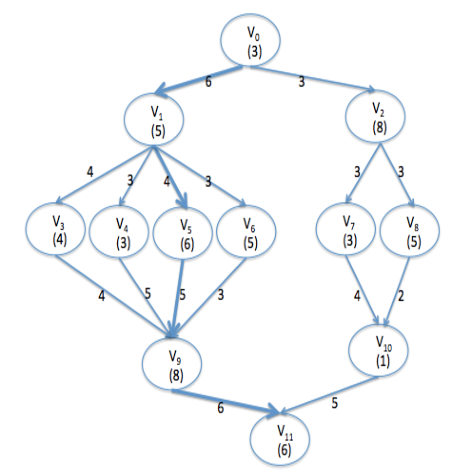
\includegraphics[width=7cm]{dag_example}
    \vspace{5pt}
	\caption{Example of a DAG representation of workflow}
	\label{fig:dag_example}
\end{figure} 

Workflow scheduling is an important aspect in workflow execution in that different scheduling algorithms might results in significant difference in makespan and resource utilization rate. The majority of these algorithms take advantage of the concept of critical path (CP), which is the longest path of the DAG representing the workflow. For a given DAG, the critical path represents the theoretical minimum time needed to finish the execution of a workflow, which is defined by the summation of the computation costs of all tasks in the critical path (which are denoted as CP-tasks). Because of its importance effect on both performance and cost, the workflow scheduling problem in general has been extensively studied and various solutions have been proposed in the literature. Representatives of such solutions include DCP (dynamic critical path), HEFT (heterogeneous earliest-finish-time), CPOP (critical path on a processor), CPF (critical path first). The majority of these studies focus either on minimizing makespan within the resource capacity available, or minimizing cost by reducing the number of nodes needed to run the workflow with a acceptable makespan. 

DCP -- Kwok et al. \cite{kwok1996dynamic} propose DCP, which assigns a task considering the critical path of partial schedule. DCP implicitly prevents the excessive (most likely unnecessary) use of processors in that for non-CP tasks it only considers processors already used in the schedule. 

HEFT / CPOP -- Topcuoglu et al. \cite{topcuoglu2002performance} present HEFT and CPOP for a bounded number of heterogeneous processors with an objective to simultaneously meet high performance and fast scheduling time. The HEFT algorithm selects the task with the highest upward rank value at each step and assigns the selected task to the processor, which minimizes its earliest finish time with an insertion-based approach. The CPOP algorithm uses the summation of upward and downward rank values for prioritizing tasks. Another difference is in the processor selection phase, which schedules the critical tasks onto the processor that minimizes the total execution time of the critical tasks. To compare HEFT and CPOP with other workflow scheduling algorithms, the authors designed a parametric graph generator to generate weighted directed acyclic graphs with various characteristics. The result shows that HEFT and CPOP can achieve shorter makespan with small cost.

PCP -- Abrishami et al. \cite{abrishami2012cost} proposed the partial critical path algorithm to minimize cost while trying to meet the user-defined deadline of a given workflow, taking advantage of the negotiable pricing mechanism of utility grids. For a given workflow, the algorithm first assigns sub-deadlines to CP tasks and to remaining tasks based on deadlines of CP tasks. Then the algorithm schedules tasks in the cheapest service that can satisfy the sub-deadline constraints. 

CPF -- Lee et al. \cite{lee2013stretch} proposed the critical path first algorithm with the assumption of resource abundance in a public cloud environment. The CPF algorithm first stretches out the schedule to proactively preserve critical path length, which is the shortest possible time of completion, then compacts the schedule for resource efficiency by rearranging tasks making use of idle/inefficiency slots present in the schedule. With this two-step approach CPF optimizes both the makespan and the resource utilization rate.

In general, the workflow scheduling problem has been studied extensively and thoroughly, with various solutions pushing both performance and cost to their limits. Unless there emerges a new form of computing resource that can be leveraged by workflow, there exists very little space for improvement in workflow scheduling.

\section{Workflow Execution Frameworks}
\label{sec:workflow_execution_frameworks}


A large-scale workflow application is usually run in a cluster with multiple nodes, with hundreds and even thousands of tasks with data and priority dependencies. The execution of a workflow involves multiple repeating steps including job scheduling, resource reservation and provisioning, data staging, job execution, status update, and fault tolerance. As scientific workflows are becoming increasingly large-scale and complex, their distributed execution across multiple resources is far beyond an average task. Due to the complexity of the workflow execution process, various workflow execution frameworks have been developed to automate this process. Some of the popular workflow execution frameworks being used in large-scale scientific computing include Condor \cite{couvares2007workflow} \cite{litzkow1988condor}, Pegasus \cite{deelman2004pegasus}, Kepler \cite{altintas2004kepler}, Taverna \cite{oinn2004taverna}, Trident \cite{barga2008trident} \cite{simmhan2009building}[21], Apache Airavata \cite{marru2011apache}, and Polyphony \cite{shams2010polyphony}. 

Condor is one of the earliest versions of workflow execution framework. Originally it was designed to harvest idle computing resource by scheduling jobs to idling UNIX workstations. With techniques such as local shadow process, job checkpointing and migration, and fair access to remote cycles, Condor was able to schedule and execute jobs utilizing idling computing resource with minimum impact on local user activities, as well as protecting the rights of light users against heavy users. Gradually Condor evolves into a feature-reach workflow execution framework, with a focus on high-throughput computations. In particular, the DAGMan module in Condor has been widely adopted by the scientific-computing community.

Pegasus stands for Planning for Execution in Grids. It is a workflow execution framework that can map complex workflows onto the Grid. Pegasus takes an abstract description of workflow in the form of a DAG, and finds the data and computing resource that are capable of executing the workflow, resulting in an executable workflow which is denoted as the concrete workflow. In the concrete workflow all jobs are bound to specific Grid resources, with necessary utilities to stage data in and out of the execution environment. Pegasus was released as part of the GriPhyN Virtual Data Toolkit, and has been used in a variety of applications ranging from astronomy, biology, gravitational-wave science, and high-energy physics.

Kepler was built upon Ptolemy II, a dataflow-oriented workflow execution framework, with some advanced extensions. In Kepler, a director module controls the execution of a workflow, while individual jobs and data transfer are implemented as reusable actors representing data source, sinks, data transformers, analytical steps, or arbitratory computational steps. Kepler provides an intuitive GUI with which scientists can easily design, prototype, execute, and analyze reusable scientific workflows. The web and grid service actor in Kepler allows scientists to utilize computation resources on the network, especially scientific computing grids. Kepler actors can be local Java threads (default), distributed execution threads via web and grid services, or libraries written in other languages invoked via Java Native Interface (JNI). Kepler acts as an agent between the computing infrastructure (such as grid, cluster, web services, data transfer) and the scientists, allowing scientists to focus on their own problem domain. 

Taverna was developed as a tool for the composition and enactment of bioinformatics workflows for the life science community. In Taverna, scientists can define their workflows in a domain-specific language called the simple conceptual unified flow language (Scufl), in which each step in the workflow represents on atomic task. Taverna provides a GUI with which scientists can composite workflows without learning the Scufl language. With the increasing number of bioinformatics databases and computational programs being made available as web services, Taverna enables researchers to take full advantages of such resources by automating the data searching and data staging processes for workflow execution. In a similar fashion, the Scufl workflows created using Taverna are resources in their own right that can be shared among scientists. 

Trident is a scientific workflow workbench built on top of Windows Workflow Foundation, a commercial workflow enactment engine designed for the Windows operating system. The Trident registry serves as a catalog of known data sets, services, workflows and activities, and compute resources, as well as maintaining state for all active workflows. Trident include a visual workflow composer in which scientists can author a workflow using the above-mentioned existing components from the service catalog. Trident also has a web portal, which allows scientist to launch and manage workflows from any location that has an Internet connection. One of the innovations in Trident is a data access layer that abstracts the actual storage service used from the workflows. So a workflow can read and/or write data objects that are transparently mapped to the target data source. Currently Trident supports a default XML store and SQL Server for local storage, and Amazon S3 and SQL Azure Data Services for Cloud storage. The fact that Trident is tightly bound to the Windows operating system makes it less appealing to scientists, which prevents its adoption in the scientific workflow community.

The Apache Airavata project was initiated to create an open development community - not just open source software - for workflow researchers. During the past researchers have created numerous toolsets and utilities for workflow research in the form of open source software. However, due to the lack of a cohesive open community, other researchers are either not aware of the availability of these tools, or are not able to evaluate the merits of these tools without extensive testing, resulting in the re-creation of similar features or functionality. The goal of the Apache Airavata project is to mitigate such continuous reinvention by fostering an open development community. The core features of the Apache Airavata project include (a) desktop and browser-based user interface; (b) server side workflow scheduling and execution framework; and (c) interoperability with third party data, workflow, and management tools. Other innovative features of the Apache Airavata project include integration with Apache Hadoop, a scalable and distributed infrastructure for big data analysis.

Polyphony is the first scientific workflow execution framework designed with the principles of cloud computing. All previous scientific workflow execution frameworks are designed with a known set of computing resources, and try to map computing tasks to available computing resources with the goal to minimize makespan. Such a design philosophy naturally lead to the master-slave architecture with stateful implementations. The workflow execution framework acts as the master assigning tasks to the computing slaves, as well as data staging and keeping tract of the status of nodes, tasks, and data. Such workflow execution frameworks favor homogeneous computing environments in which all computing nodes have similar configurations in terms of CPU, memory, and storage. Polyphony, on the contrary, takes a publisher/subscriber approach. In Polyphone, a workflow scheduling module publishes tasks to be executed to a distributed queue in the form of messages when the data dependencies are met. Multiple worker nodes can subscribe to the queue pulling tasks to be executed, and uploading the output data to the desired location based on the instructions given by the message obtained from the queue. The workflow scheduling module dynamically examines the execution progress of the whole workflow, and publishes new tasks that meet data dependencies to the queue. With such a design Polyphony does not have a central module trying to keep tract of any or all the nodes, and does not even need to have any knowledge about the configurations of the nodes. In fact, the worker nodes are not being managed in any way, and do not have any status to maintain. Any computer - Linux servers, personal laptops, cloud instances, or supercomputers - can install a software application to become and worker node and check out tasks from the distributed queue, process the task and return the output to the desired storage services, such as NFS and Amazon Simple Storage Services (S3) . In order to integrate an application into the Polyphony framework, developers will need to write a module and include it in the Polyphony distributions to be installed onto the worker nodes. 

As we can see, the majority of existing scientific workflow execution frameworks are designed with a known set of computing resources, and try to map computing tasks to available computing resources with the goal to minimize makespan. Polyphony, on the other hand, distributes tasks with a queue with the assumption that worker nodes are abundant and will automatically check out and process the tasks. These two cases represent two extreme situation in scientific computation - resource constraint in a grid environment and resource abundance in a public cloud environment. These is another situation that has not been supported by any existing workflow execution framework - a dynamical environment where the number of worker nodes is changing to address resource utilization and cost constraints in public clouds. For example, for a long running complex scientific workflow, the demand for computing resource varies at different phase of the computation. When there are a lot of parallel tasks it might be needed to spin up more worker nodes to reduce makespan. When there are only a few long running tasks it might be needed to shut down some worker nodes to reduce resource consumption. The demand for such dynamic scaling support might not seem to be very attractive with the hourly billing plan provided by AWS, but makes more sense with more fine-grained billing mechanisms such as the per-minute billing plans provided by Google Compute Engine (GCE) and Windows Azure.  

All existing scientific workflow execution frameworks focus heavily on the composition and execution of the workflow, but offers very limited capabilities in the post-processing of the workflow. The workflow scheduling and execution traces are usually written to a text file, in most cases in XML format. For a large-scale workflow with thousands of tasks, scientists can only calculate the overall resource utilization such as the total or percentage amount of time being used for computation and data staging, but the details about the scheduling and execution are often overwhelmed by the size of the output. It would be helpful for scientists - especially workflow researchers - to have a tools that can visualize the resource utilization status of all worker nodes during the whole makespan. Such a tool can provide insights into the idling time slots in the computing environment, which will help researchers design better workflow scheduling algorithms or resource allocation strategies.

\section{Workflow Execution in the Cloud}
\label{sec:workflow_execution_cloud}

In recent years, cloud computing is gaining increasing adoption in the scientific computing community. The seemingly unlimited computing resource is very attractive to researcher, who have long suffered resource deficit with the computing facilities they have access to. It is important to note that the expense of using 1000 worker nodes for 1 hour is the same as the expense of using 1 worker node for 1000 hours in a public cloud. This is a crucial benefit to any application; expediency of computational result comes for free simply due to the elasticity available in the cloud.

Early studies on doing scientific workflows on public clouds tried to determine the benefits and drawbacks of cloud computing for scientific applications, with a focus on performance and cost. Juve et al. \cite{juve2009scientific} examine the performance of doing scientific workflow in Amazon EC2 using three characteristic workflows - Montage, Broadband, and Epigenome - and compare the result with a typical HPC system built with the NCSA`s Abe cluster. The results indicate the primary advantage of Abe is the availability of a high-speed interconnect, as well as a parallel file system that significantly improve the performance of I/O-intensive applications. In fact, the performance of EC2 instances is very close to that of Abe when  the Abe cluster is using the local disks for storage. The primary cost of doing scientific workflows on public clouds lies in acquiring resources to execute workflow tasks. The storage cost is relatively small, and data transfer cost can be reduced by storing data in the cloud rather than transferring it for each workflow.

Juve et al. \cite{juve2010data} \cite{juve2012evaluation} further investigate the I/O problem associated with doing scientific worflows on public clouds, exploring various data sharing options on Amazon EC2. In grids and HPC clusters, workflow data is often stored on network and parallel file systems, which are not available in public clouds. The authors investigate ways to store and share data for scientific workflows in the cloud, including Amazon S3, NFS, GlusterFS, and PVFS. Experiments are carried out with three characteristic workflows - Montage, Broadband, and Epigenome. The results indicate that GlusterFS delivers good performance for all the applications tested and seems to perform well with both a large number of small files. NFS performs well when the number of clients is small or the workload is not I/O-intensive. Both PVFS and S3 perform poorly on workloads with a large number of small files. In general, the storage systems that produce the best workflow runtimes result in the lowest cost.

Deelman et al. \cite{deelman2008cost} study the cost of running scientific workflows on the cloud with various compute, storage, and communication options. Using the Montage application and Amazon EC2 as a case study, the authors determine that for a data intensive application with a small computational granularity, the storage costs is insignificant as compared to the computation cost. Other researchers, such as Juve et al. \cite{juve2009scientific} \cite{juve2010data} \cite{juve2012evaluation}, also agree that cloud computing offers a cost-effective solution for scientific workflow applications.

Computing resources on public clouds, as well as scientific grids, should be considered as fragile where faults are likely to occur. In Amazon EC2, a user`s VM instances might be terminated because of a fault on the underlying server hardware. Without sophisticated fault handling, workflows are frequently abandoned when a fault occurs, leading to a waste of computing resource. Ramakrishnan et al. \cite{ramakrishnan2009vgrads} study the execution of time-sensitive scientific workflows on the cloud with special considerations on fault tolerance. Probabilities of tasks completing are computed using the failure probability of the computing resource and the failure probabilities of its parent tasks. To increase the probability of success for each workflow task, the workflow planner interacts with a fault tolerance component to determine if a task should implement replication. Juhnke et al. \cite{juhnke2009fault} propose a fault tolerance module to be used with ActiveBPEL, an open source workflow enactment engine, to handle infrastructure faults for long-running workflows. By pre-classifying the possible faults in the infrastructure, policies are configured to invoke automatic recovery by providing redundancy resources using public clouds such as Amazon EC2. As compared to \cite{ramakrishnan2009vgrads} and \cite{juhnke2009fault}, which involves complicated techniques in determining the status of both the infrastructure and the tasks, the Polyphony workflow execution framework \cite{shams2010polyphony} offers a much more elegant solution to the fault tolerance problem using characteristics of the Amazon Simple Queue Service (SQS). In Polyphony, tasks are published to a distributed queue, while worker nodes actively pull the queue to check out tasks for processing. Once a task has been checked out by a worker node, it becomes invisible to other worker nodes within a certain timeout period. When the worker node finish processing the task, it uploads the output to the desired storage service, and deletes the task from the queue. If the task has not been deleted from the queue after the timeout period, which is an indicator that the task has not been successfully processed, it becomes visible to all worker nodes again, and can be checked out and processed by other worker nodes. With such a mechanism any worker nodes can fail at any time without affecting the successful execution of the workflow.

Traditionally, workflow scheduling focuses on the minimization of makespan with tightly coupled computer systems like clusters. When moving to the public cloud environment, scientists usually pre-allocate a certain number of VM instances so that they can execute workflows in a way similar to traditional clusters. Because of the data dependencies and priorities of the tasks, it is inevitable that some worker nodes might be idling for a considerably long period of time during the execution. This represents further cost optimization opportunities in that scientists can terminate instances that are waiting for tasks to be available, and launch instances when additional computing resource is needed. Dornemann et al. \cite{dornemann2009demand} present an on-demand resource provisioning solution for BPEL workflows using Amazon EC2. Experiments are carried out with the ActiveBPEL workflow enactment engine and computational intensive video analysis applications to verify the visibility of the solution. Ostermann et al. \cite{ostermann2010dynamic} study some specific techniques for dynamically provisioning computing resource on Amazon EC2 for scientific workflows, including cloud start, instance type, grid scheduling, and cloud stop. Nagavaram et al. \cite{nagavaram2011cloud} presented a case study using a dynamic workflow for mass spectrometry data analysis on Amazon EC2. In order to effectively use cloud resources, researchers parallelize the search method in MassMatrix, an application which searches proteins and peptides from tandem mass spectrometry data. A flexible workflow was created with the Pegasus to guide the data analysis process. Finally, a dynamic resource allocation module (an extension of Pegasus/Wrangler) was created to launch or terminate VM instances based on a time constraint specified by the user. Experiments with several different datasets indicate that this technique scales quite well, and is effective in meeting time constraints. One other aspect, although not explicitly emphasized by the authors, is that rewriting some critical components of the tasks (such as the search method in MassMatrix) is needed to take full advantage of public clouds. 


\section{Research Directions}
\label{sec:research_directions}


This literature review makes the following observations regarding researches on scientific workflows:

Workflow scheduling algorithms have been studied extensively, with only very limited space in workspan optimization.  This is particularly true with a traditional computer cluster where the total amount of computing resource is pre-allocated and does not change over the makespan. However, in a public cloud environment where computing resource is abundant, there exist opportunities for cost optimization with dynamic resource allocation and termination. There have been some research efforts exploiting dynamic resource allocation on Amazon EC2, which offers an bill-by-hour mechanism. New public clouds - such as Google Compute Engine and Windows Azure - are offering bill-by-minute mechanism. Such a finer grained billing mechanism represents further cost optimization opportunities, and deserves the attention from the scientific workflow research community.

In the past, resource scarcity was a great challenge for the scientific computing community. Most researchers depend on grid computing to obtain access to large scale computing resource. In a grid environment, researcher are confronted with resource heterogeneity in compute, networking, and storage. In recent years, public clouds are gradually making their way into the scientific computing community and gaining increasing level of adoption. As compared to a grid environment, a public cloud offers seemingly unlimited amount of computing resource where a large scale homogeneous computing environment can be constructed on demand. Despite the significant difference between the grid environment and the public cloud environment, many researchers in the scientific workflow community continue to use methodologies and tools developed for grid computing in public clouds. This results in significant resource under utilization as well as over spending. 

In order to utilize public clouds in a more cost-effective way, further research is needed in the following directions:

(1) How do we optimize the execution of scientific workflows in public clouds?

(2) Can we use existing tools and methodologies directly in public clouds, or new tools and methodologies are needed for public clouds?

(3) How do we optimize the execution of large-scale scientific workflow ensembles in public clouds to meet both cost and deadline constrains?





\chapter{Optimizing the Execution of Large Scale Scientific Workflows in Public Clouds}
\label{chapter:dewe_v1}

\section{Introduction}
\label{sec:dewe_v1:dewe_v1_intro}

In recent years, the concept of workflow has gained increasing level of acceptance by the scientific computing community. Large-scale scientific computations usually involve a large number of different tasks, often in the number of hundreds or thousands. Some of these tasks depend on the output of other tasks (i.e., precedence constraints), forming a workflow. When the precedence requirements for certain tasks have been met, each of these tasks can then run independently in its own environment. In practice, scientific workflows are usually run on clusters with multiple computing nodes. A workflow management system is needed to control the sequence of task execution, computing resource assignment, as well as data transfer to satisfy the precedence constraints. 

Examples of scientific workflows are Montage \cite{montage, web:montage}, LIGO \cite{ligo}, and CyberShake \cite{cybershake}. Examples of workflow management systems are Pegasus \cite{deelman2004pegasus} and Kepler \cite{altintas2004kepler}.

For many scientific workflow applications, the task modules are often developed as sequential code. One reason is that these modules were developed in early years when the concept of parallel programming had not been widely adopted by researchers in specific problem domains. Even today the development of parallel code is pretty complex for non experts in parallel programming. The other reason is that workflow management systems usually use CPU slots (e.g., cores, or virtual CPU cores or vCPUs) as basic resource allocation units, and it is easier to carry out workflow scheduling with a one-to-one mapping between CPU slots and tasks. Due to the precedence constraints between tasks, only certain tasks are eligible to run at a given point in time. When the number of concurrently running tasks is smaller than the number of CPU slots available in the computing cluster, the extra CPU slots will be idling. In the extreme case, only one task is running on one CPU slot in a large computing cluster, resulting in significant under-utilization of computing resources.

A workflow can be represented by a directed acyclic graph (DAG), where the vertices represent the tasks and the edges represent the precedence constraints. The DAG scheduling problem is NP-complete in general. In recent years, there emerged a large volume of literature on workflow scheduling, with the goal to decrease the time needed by the workflow or minimize the size/cost of the computing cluster. Other attempts to optimize workflow execution include using alternative data storage and data staging options for improved I/O efficiency. However, none of the existing methods addresses the resource under-utilization problem caused by sequential code, especially when certain sequential code becomes the bottleneck of a workflow. 

In this chapter, we present a set of methods to optimize the execution of scientific workflows, with the Montage astronomical mosaic engine running on Amazon EC2 as an example. We use our own DEWE (Distributed Elastic Workflow Execution)\footnote{DEWE including its source code and visualization toolkit used in this study is available from \url{https://bitbucket.org/lleslie/dwf/wiki/Home}.} as a workflow management system. The main contributions of the present work are:

\begin{itemize}
%	\item We compare the impact of compiler optimization on the performance of the Montage workflow, using both GNU C Compiler (GCC) and Intel C Compiler (ICC).  
	\item We develop a workflow visualization toolkit to visualize the workflow execution process and resource consumption pattern. We use the workflow visualization toolkit to process the trace files produced by the workflow management system to identify the bottleneck of the Montage workflow.
	\item We use parallelization techniques to optimize the mBgModel module in the Montage workflow, resulting in significant degree of performance gains.
	\item We compare the impact of different computing cluster configurations on Amazon EC2 on the performance of the Montage workflow, and analyze the root cause for the performance difference. 
\end{itemize}

The rest of this chapter is organized as follows. Section \ref{v1_sec:visualization} describes the design of the workflow visualization toolkit and its usage. In Section \ref{v1_sec:parallel}, we first discuss the impact of compiler optimization on performance and then use code level parallelization to mitigate the bottleneck. In Section \ref{v1_sec:eval}, we evaluate our optimization approach by comparing different cluster configurations on Amazon EC2. We summarize our conclusions in Section \ref{v1_sec:summary}.

\section{The Montage Workflow}
\label{v1_sec:montage}


\begin{figure}[!t]
	\centering
	\hspace{-10pt}
	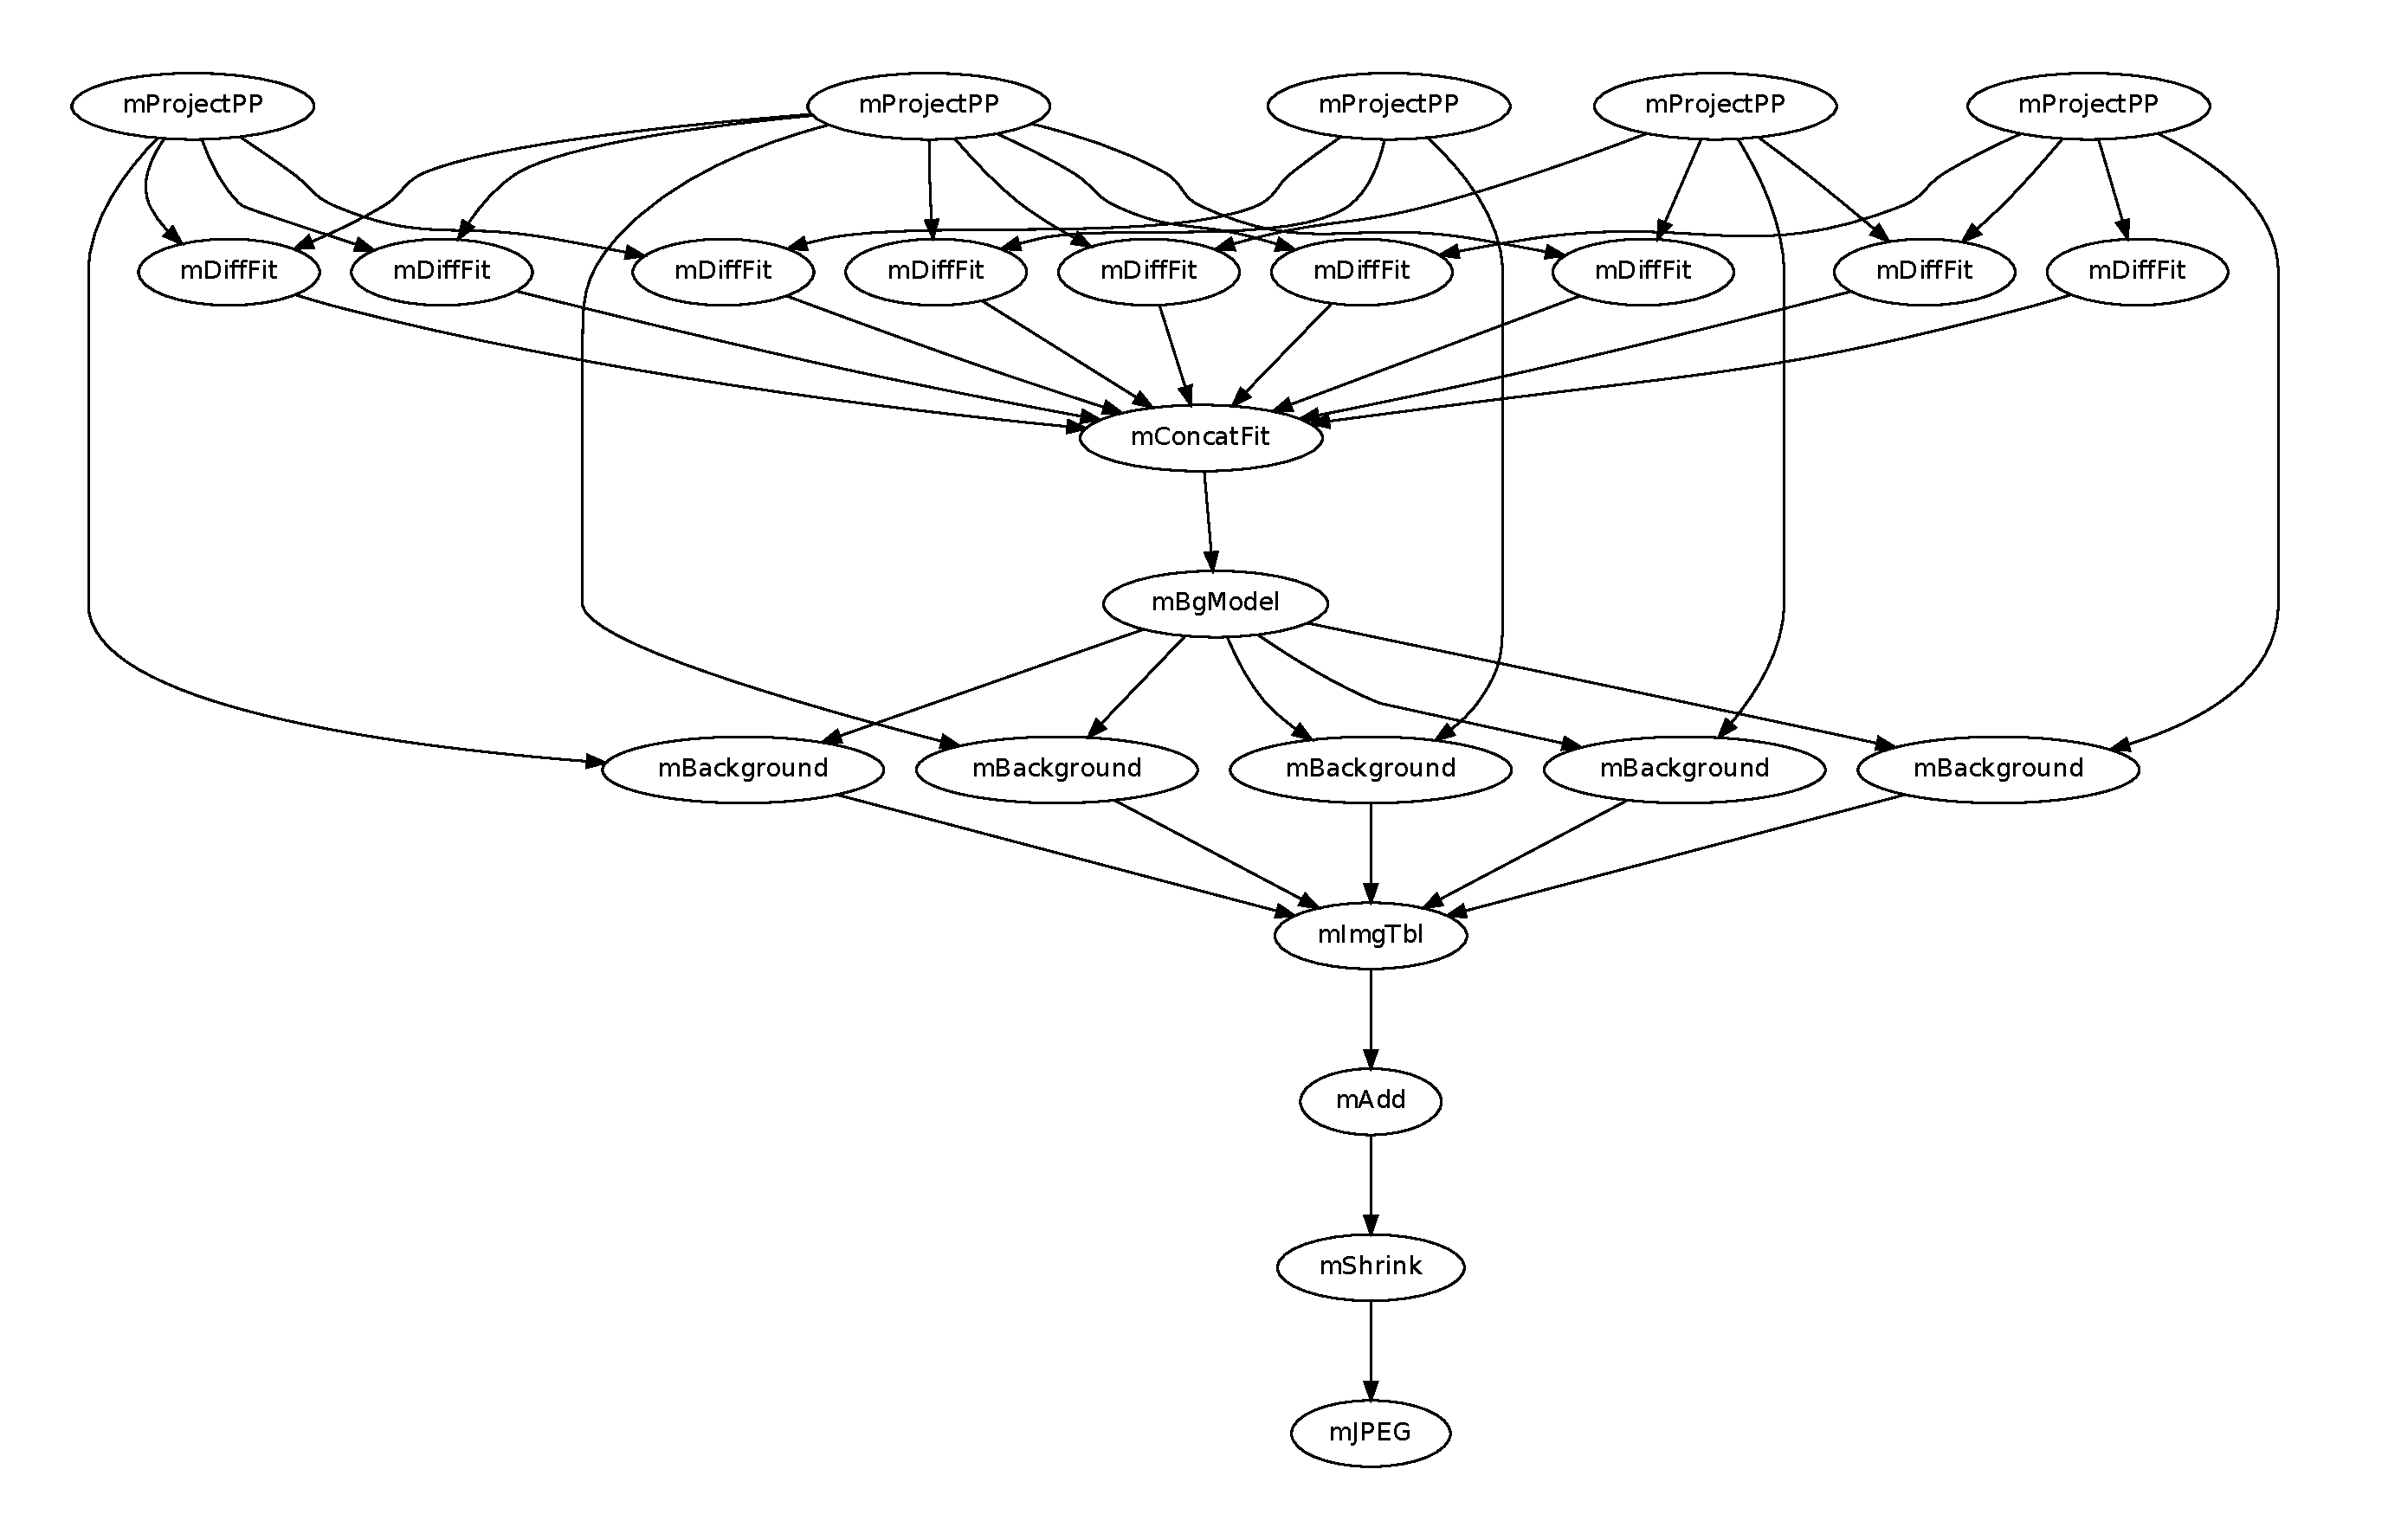
\includegraphics[width=9.7cm, height=7cm]{montage}
    \caption{The structure of the Montage workflow.}
    \vspace{-10pt}
	\label{v1_fig:montage}
\end{figure}


In this chapter, we choose Montage as a representative example of large scale scientific workflows for our case study. Montage is an astronomical image mosaic engine that assembles individual images of the sky into a mosaic. A 6.0 degree Montage workflow creates a 6-by-6 degree square mosaic centered at a particular region of the sky (e.g., M16). The number of jobs and input data files increases with the number of degrees of the mosaic. 

Figure \ref{v1_fig:montage} describes the structure of the Montage workflow. The progress of the workflow has a three-stage pattern. During the first stage, a large number of mProjectPP jobs run in parallel, followed by a large number of mDiffFit jobs running in parallel. During the second stage, two jobs mConcatFit and mBgModel run one after another, during which no other jobs are eligible to run. In this paper, we consider mConcatFit and mBgModel as blocking jobs because they block the execution of other jobs. During the third stage, a large number of mBackground jobs run in parallel, followed by a small number of mImgTbl, mAdd, mShrink, and mJPEG jobs.

A 6.0 degree Montage workflow contains 8,586 jobs, 1,444 input files with a total size of 4.0 GB, and 22,850 intermediate files with a total size of 35 GB. In practice, a set of smaller image mosaics are needed to produce a large image mosaic, where each smaller image mosaic is generated by a Montage workflow. For example, the Galaetic Plane workflow ensemble \cite{deelman2013hosted} consists of 17 workflows, each of which further contains 900 sub-workflows. In this chapter, we are more concern about the execution of a single Montage workflow in a public cloud environment. In the next chapter, we will discuss the execution of large-scale Montage workflow ensembles in public clouds.


\section{Workflow Visualization Toolkit}
\label{v1_sec:visualization}

\begin{figure}[t!]
\centering
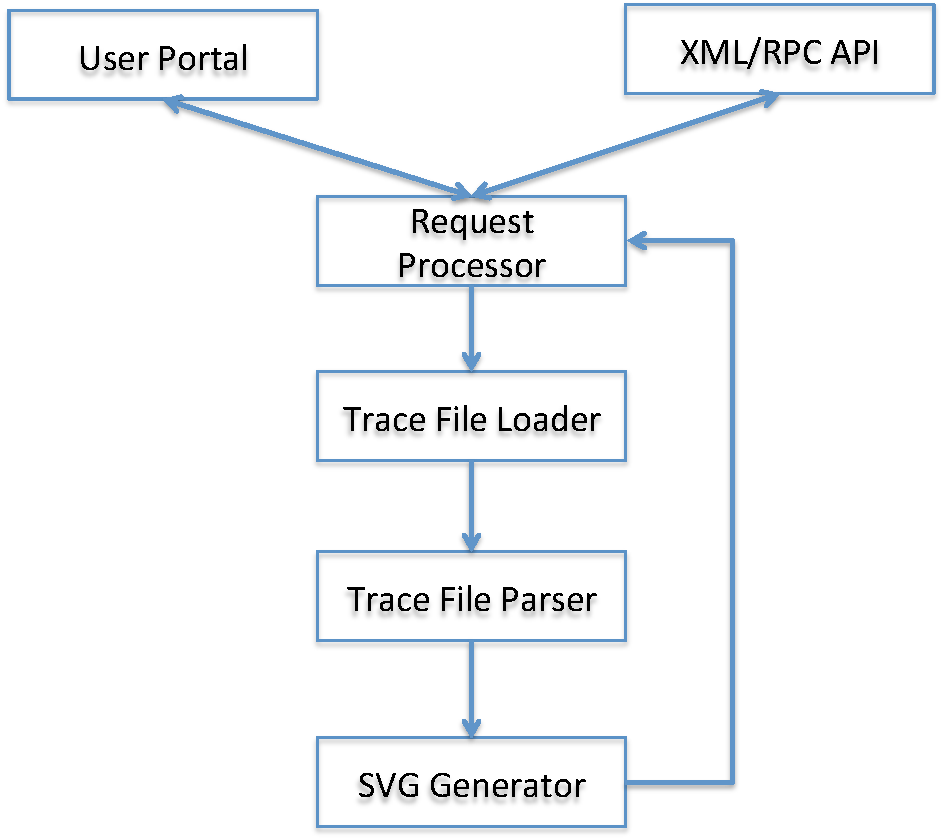
\includegraphics[width=8cm]{toolkit}
\caption{Design of Workflow Visualization Toolkit}
	\label{fig:toolkit}
\end{figure}



In this section, we present a workflow visualization toolkit that visualizes the workflow execution process and its resource consumption pattern. Figure \ref{fig:toolkit} shows the design of the workflow visualization toolkit. The user portal accepts user requests from a web browser, while the XML/RPC API accepts user requests from third party applications (such as workflow execution frameworks) via API calls. Both requests specify the type of visualization to produce, the format of the workflow trace file, the location of the workflow trace file in the form of a public accessible URL, along with some other parameters. The request handler receives these requests, and coordinates the different steps needed to produce the output vector graph. The trace file loader loads the workflow trace file from the URL specified by the user. The trace file parser extracts workflow execution information from the trace file and saves it into a data structure, as well as calculating the overall resource utilization rates for each worker node and CPU. The SVG generator produces the scalable vector graph (SVG) based on the parsed information saved in the data structure, and returns it to the request handler. The request handler then returns the output scalable vector graph to the user's browser or the third party application for further integration.

\begin{figure*}[ht]
\centering
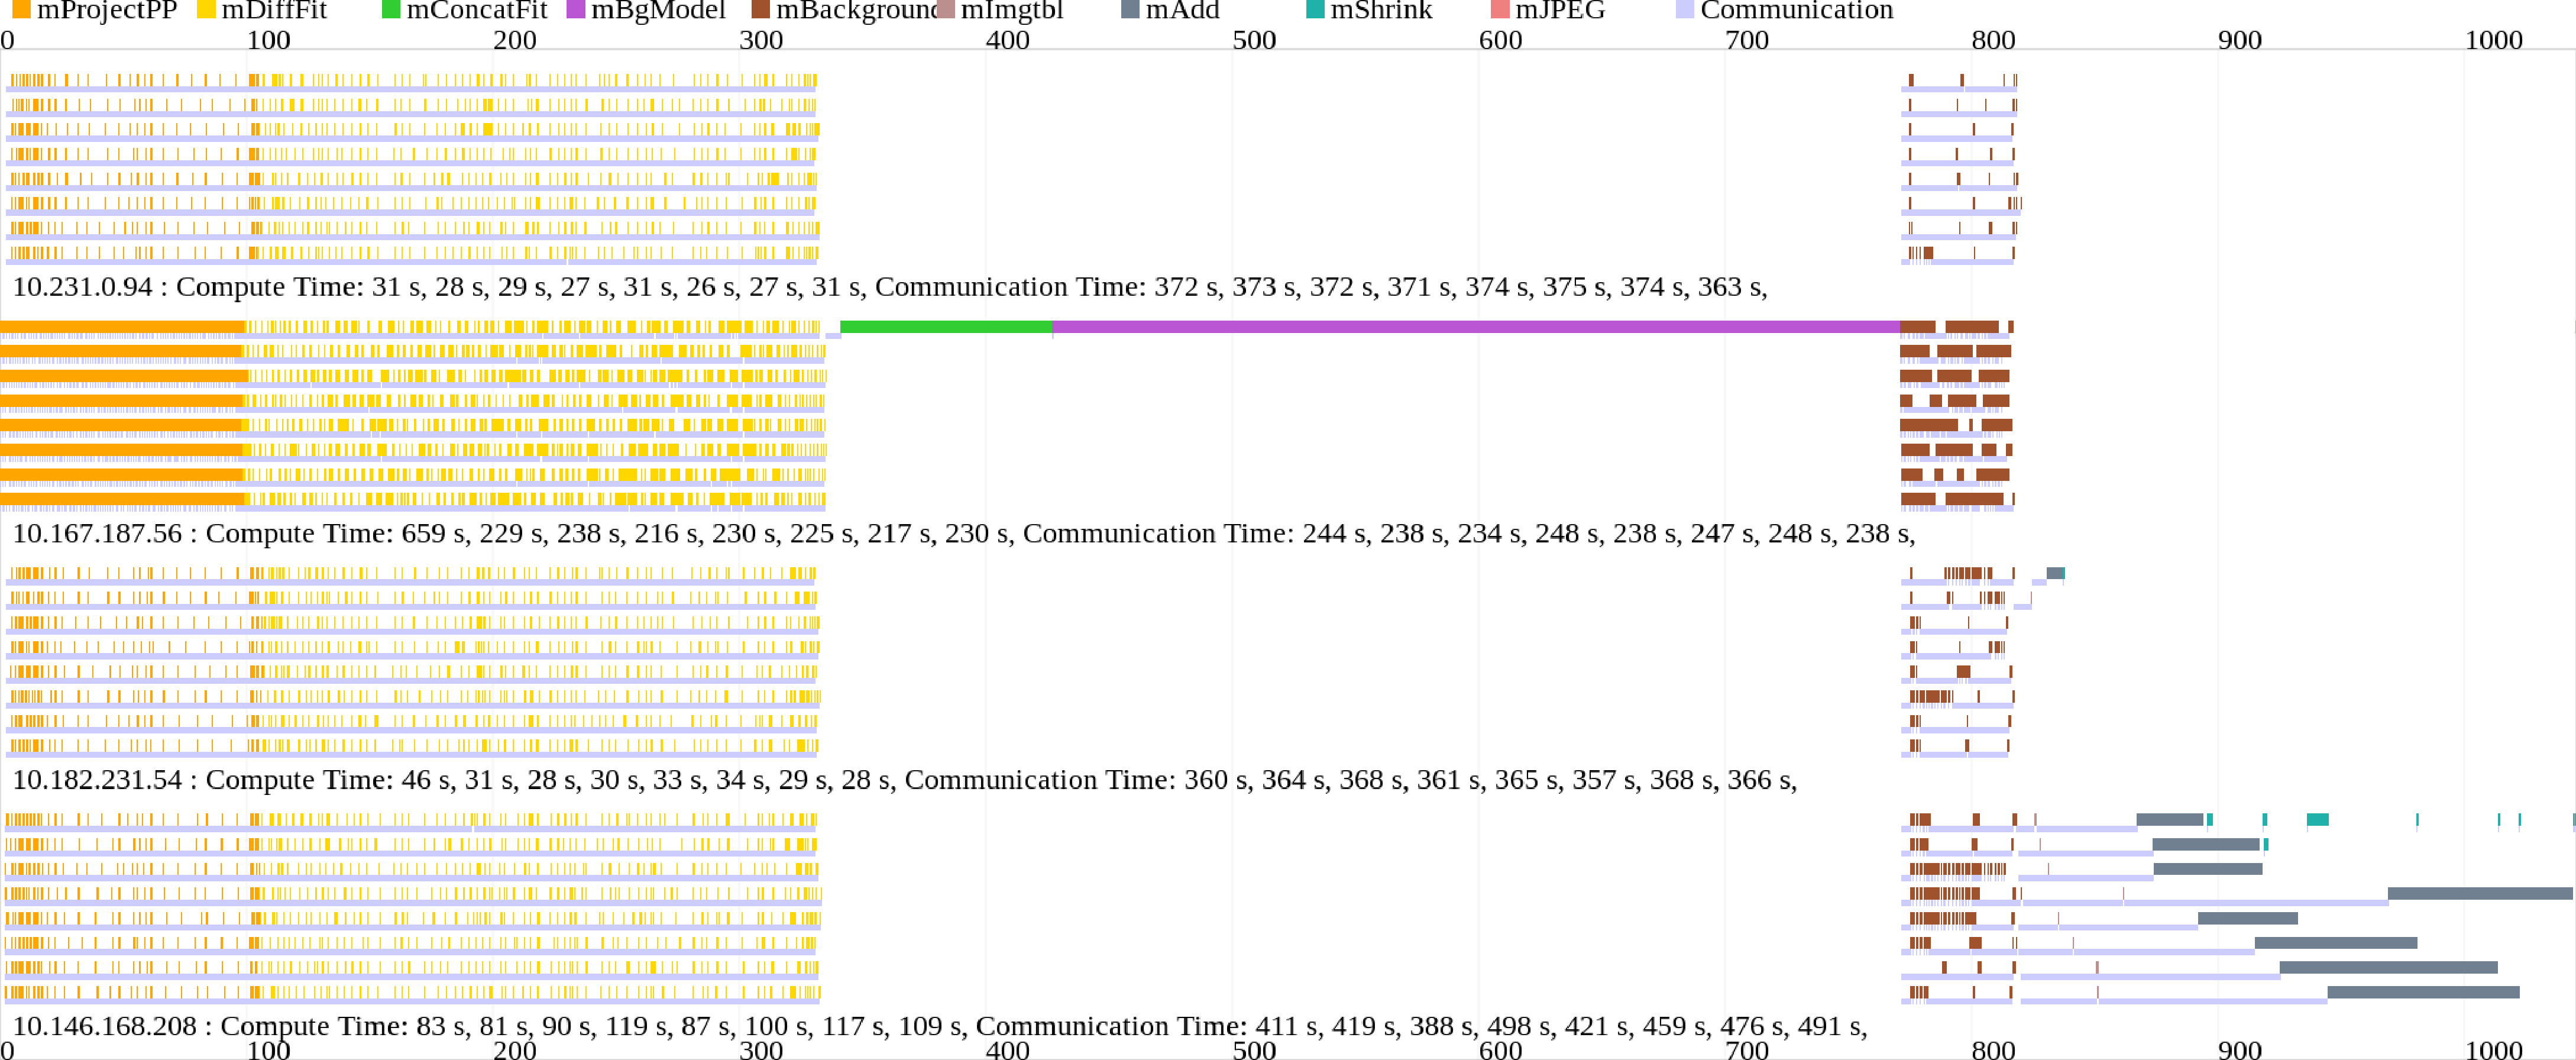
\includegraphics[width=16cm]{visual}
\caption{Detailed visualization of a 6.0 degree Montage workflow running Amazon EC2. The computing cluster includes 4 m3.2xlarge instances.}
\label{fig:detail}
\end{figure*}

\begin{figure*}[ht]
\centering
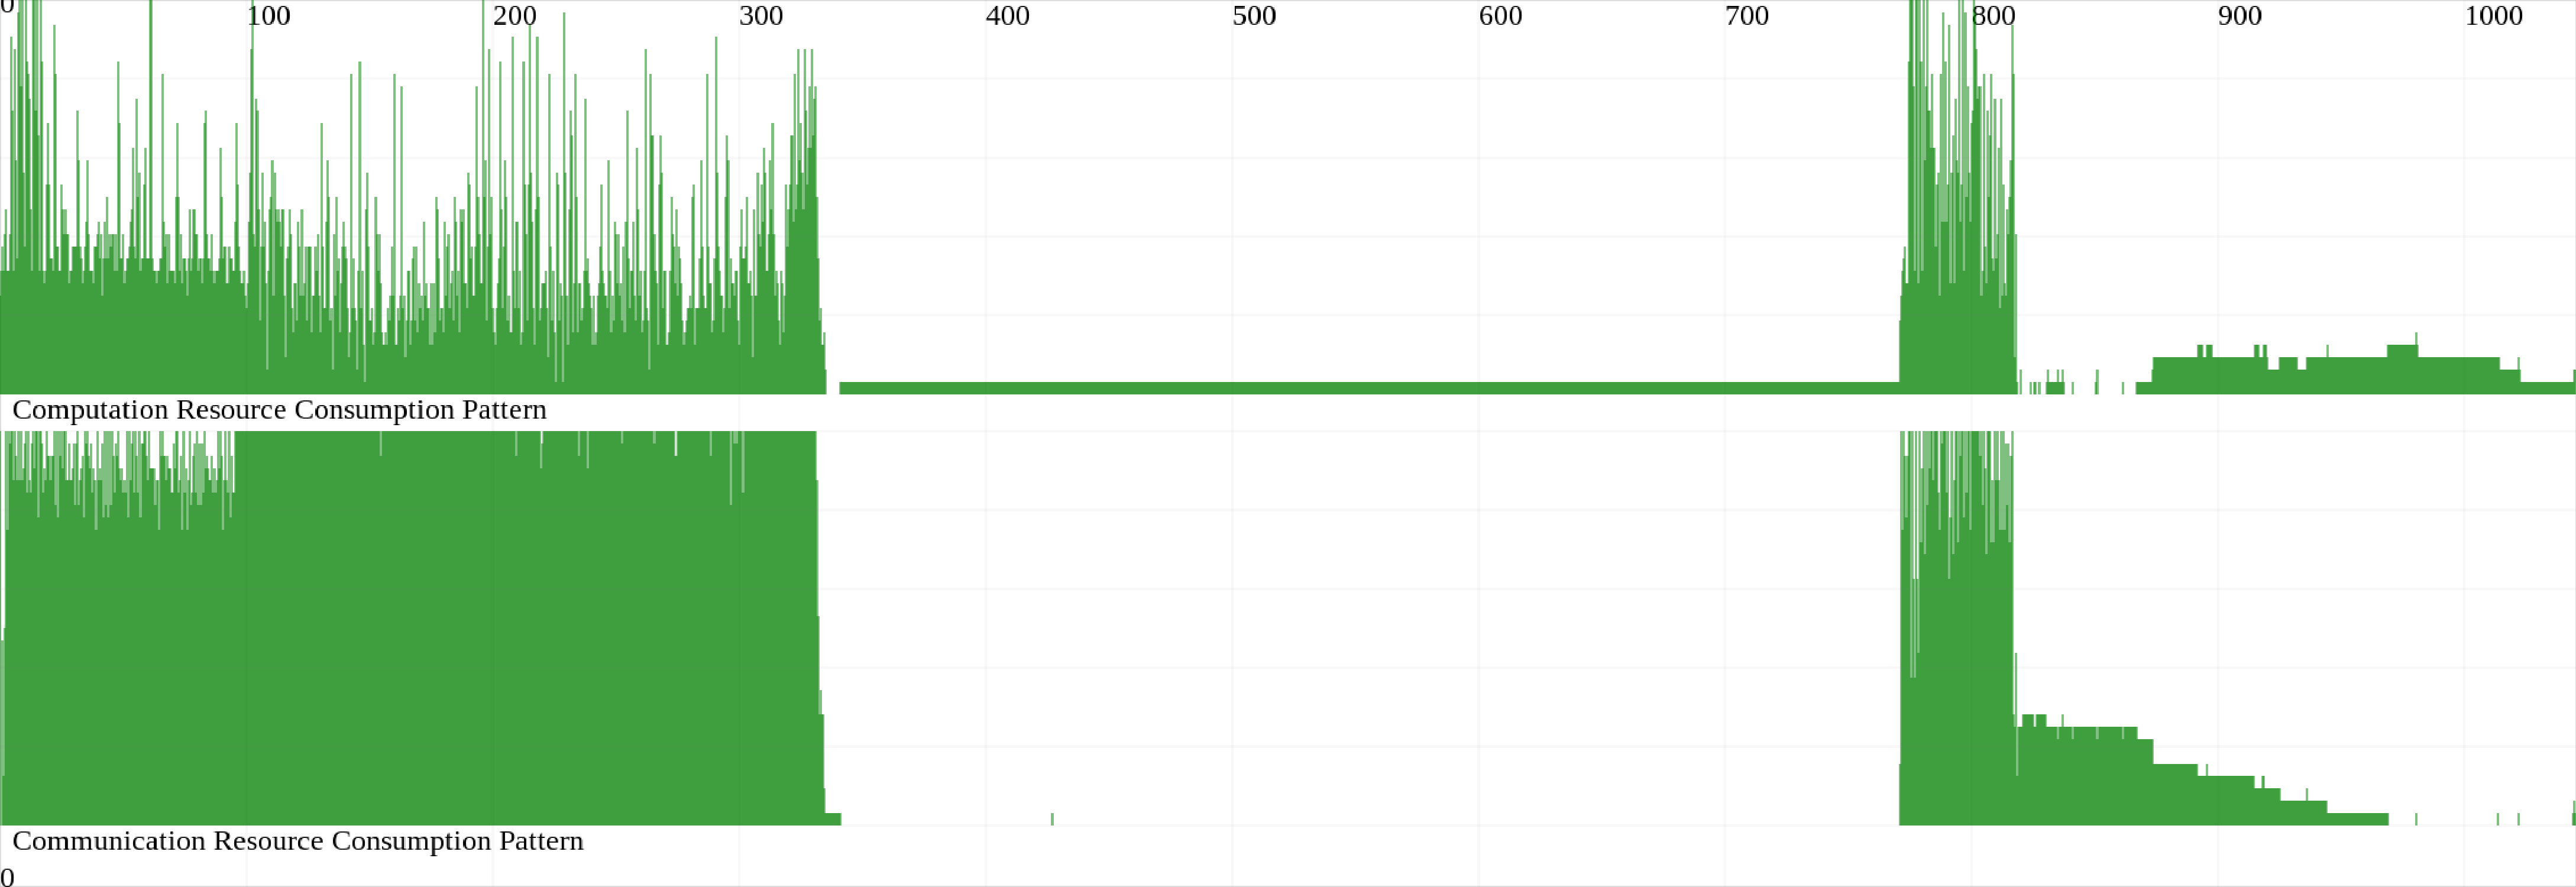
\includegraphics[width=16cm]{pattern}
\caption{Resource consumption pattern of a 6.0 degree Montage workflow running Amazon EC2. The computing cluster includes 4 m3.2xlarge instances.}
\label{fig:pattern}
\end{figure*}



The workflow visualization toolkit takes a workflow execution trace file as the input, and produces a scalable vector graph (SVG) representing the resource consumption status during the whole makespan. In a workflow execution detailed visualization (Figure \ref{fig:detail}), the scalable vector graph includes information about (a) each individual task with task coloring, such as task id, name of the binary, 
start time, task execution time, data transfer start time and data transfer execution time; and (b) summarized resource consumption information about each worker node and CPU in terms of computation time, communication time, and resource utilization rate. In a resource consumption pattern visualization (Figure \ref{fig:pattern}), the scalable vector graph provides resource consumption rate for both computation and communication resources, as defined by the ratio between the number of concurrently running computation or communication tasks and the number of total CPUs in the computing cluster.

The detailed visualization and  resource consumption patterns of a 6.0 degree Montage workflow running on Amazon EC2 are shown in Figures \ref{fig:detail} and \ref{fig:pattern}, respectively. Specifically, the computing cluster includes 4 m3.2xlarge instances, each of which has 8 vCPUs and 30 GB memory. The binaries are compiled with GCC with the -O2 compiler optimization flag. The makespan of the workflow is 1046 seconds, and the runtime of task mBgModel is 344 seconds. 


As shown in Figure  \ref{fig:detail}, and Figure \ref{fig:pattern}, the Montage workflow has a three-stage resource consumption pattern. In the first stage, a large number of mProjectPP, mDiffFit and mBackground jobs are eligible to run in parallel. These mProjectPP, mDiffFit and mBackground jobs are small jobs with very short execution time within the range of a few seconds. However, they consume and produce a large number of intermediate data files. Staging these intermediate data files between worker nodes causes significant communication cost. Considering the large number of such jobs, it is desirable to have more worker nodes to speed up the execution. However, the communication costs increases when the number of worker nodes increases, resulting in clustering performance degradation. In the second stage, a single job mConcatFit is blocking the execution of other jobs, followed by another blocking job mBgModel. The execution time of the second stage is approximately 40\% of the makespan. During this stage, among all the available computing resources only one CPU core is being utilized. When the cluster is larger, more computing resources are being wasted during this stage. In the third stage, a set of mImgTbl jobs run in parallel, followed by a set of mAdd jobs, then a set of mShrink jobs, with an exit job mJPEG to produce the final mosaic image. In this stage, as the workflow progresses towards the exit job mJPGE, the number of jobs eligible to run in parallel gradually decreases. 

As we can see, the Montage workflow ensemble represents a scheduling dilemma requiring trade-offs between cost and performance. In particular, there exists significant resource underutilization during the second stage, where only mConcatFit and mBgModel are running in a single thread fashion. In the example shown in Figure \ref{fig:detail}, the execution time for the single thread job mBgModel (344 seconds) was approximately 33\% of the total makespan (1046 seconds). Therefore, job mBgModel presents a significant opportunity for performance optimization. 


\section{Optimization Steps}
\label{v1_sec:parallel}

In this section, we study the impact of parallelization techniques on the performance of Montage. We apply standard compiler optimizations and then exploit parallelism with the support of the Parallware technology\footnote{Parallware is the new source-to-source parallelizing compiler developed by the Appentra team  (http://www.appentra.com/products/parallware/).}. 


\subsection{Compiler Optimization}
\label{sec:compiler}

The Montage workflow uses the GNU C Compiler (GCC) as the default compiler with no compiler optimization flags. To study the impact of compiler optimization on performance, we compare the performance of GCC and the Intel C Compiler (ICC). The compiler optimization flags being used include default (no optimization), -O1, -O2, and -O3. For each compiler and optimization flag combination, we carry out 3 test runs using a computing cluster of four m3.2xlarge instances\footnote{The M3 product family is the current generation general purpose product family backed by Intel Xeon E5-2670 v2 (Sandy Bridge) processors and SSD storages. The m3.2xlarge instance is the biggest instance type in the M3 product family, and each m3.2xlarge instance has 8 vCPUs, 30 GB memory, and two 80 GB SSD ephemeral storages.} in the us-east-1e availability zone, and use the average makespan as the test result. For each test run, we launch new VM instances in Amazon EC2 and setup a fresh computing cluster. These instances are terminated upon completion of a single test run. 

\begin{figure}[t!]
\centering
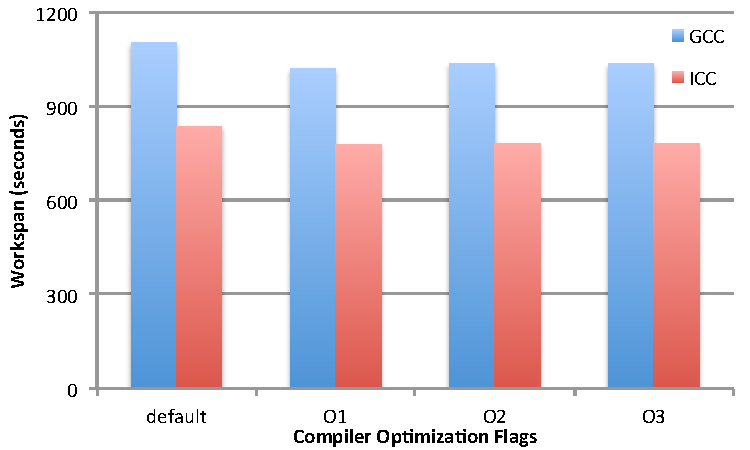
\includegraphics[width=6cm]{fig01}
\vspace{-5pt}
\caption{Compiler Optimization Results}
\vspace{-10pt}
\label{fig:compiler}
\end{figure}


Figure \ref{fig:compiler} shows the performance difference between GCC and ICC, with different compiler optimization flags. In general, ICC achieves better performance in that the makespans of the ICC test runs are 24\% shorter than the makespans of the GCC test runs. When compiler optimization flags are used, both GCC and ICC achieve additional 7\% performance gain as compared with the default version, while the difference between different compilation flags is very small.

\subsection{The Parallelization of Bottleneck Task}
\label{v1_sec:parallware}

As mBgModel is identified as the bottleneck of Montage in Section \ref{sec:visualization}, we present a cost-effective OpenMP-enabled parallelization strategy of mBgModel. For this purpose we use the technology of Parallware. The resulting OpenMP-enabled parallel mBgModel provides good performance gains at the cost of short development times. 

The Figure~\ref{fig:mbgmodel:sequentialcode} shows a pseudocode of the sequential code of the task mBgModel. 


\begin{figure}[ht]
\centering
\begin{lstlisting}
struct FitInfo {
  double a, b, c;
  ...
  struct CorrInfo *plusimg;
  struct CorrInfo *minusimg;
} *fits;

struct CorrInfo {
  double a, b, c;
  double acorrection, bcorrection, ccorrection;
  ...
  struct FitInfo **neighbors;
} *corrs;

#pragma omp parallel shared(...) private(...)
{
for (t = 0; t < niterations; t++) {
  #pragma omp for schedule(static,1)
  for (i = 0; i < ncorrs; i++) {
    corrs[i].acorrection = 0;
    corrs[i].bcorrection = 0;
    corrs[i].ccorrection = 0;
    ta = 0;
    tb = 0;
    tc = 0;
    for (j = 0; j < neighbours[i]; j++) {
      ta += corrs[i].neighbors[j]->a;
      tb += corrs[i].neighbors[j]->b;
      tc += corrs[i].neighbors[j]->c;
    }
    corrs[i].acorrection = ta/2;
    corrs[i].bcorrection = tb/2;
    corrs[i].ccorrection = tc/2;
  }
  #pragma omp for
  for (k = 0; k < ncorrs; k++) {
    corrs[k].a += corrs[k].acorrection;
    corrs[k].b += corrs[k].bcorrection;
    corrs[k].c += corrs[k].ccorrection;
  }
  #pragma omp for
  for (l = 0; l < nfits; l++) {
    fits[l].a -= fits[l].plusimg->acorrection;
    fits[l].b -= fits[l].plusimg->bcorrection;
    fits[l].c -= fits[l].plusimg->ccorrection;
    fits[l].a += fits[l].minusimg->acorrection;
    fits[l].b += fits[l].minusimg->bcorrection;
    fits[l].c += fits[l].minusimg->ccorrection;
  }
}
}
\end{lstlisting}
\vspace{-10pt}
\caption{Pseudocode of the sequential code of the task mBgModel.}
\vspace{-20pt}
\label{fig:mbgmodel:sequentialcode}
\end{figure}
%
The original source code consists of 1051 source lines of codes, according to the SLOCCount utility. The design of the data structure poses a challenge on detection of parallelism because it consists of a recursive {\em struct FitInfo}, with indirect recursion through the auxiliary {\em struct CorrInfo}. The code processes a set of astronomical images. The pixels of an astronomical image are represented as an array {\em fits[]}, and their neighbours in other images are represented in the array {\em corrs[]} and its field {\em neighbors[]}.

The algorithmic structure of the sequential mBgModel code consists of a main loop {\em for(t)} that computes {\em fits[]} and {\em corrs[]} during a fixed number of iterations {\em niterations} (line 23). In a given iteration, the values of {\em corrs[]} are updated (lines 25-46) by adding the previous value and the value of an expression that depends on {\em fits[]} through the array of {\em neighbors[]}. In addtion, the computation of {\em fits[]} is also updated (lines 48-55) with the new values of {\em corrs[]} computed at the beginning of each iteration. Thus, the main loop computes two mutually dependent variables {\em fits[]} and {\em corrs[]} that prevent parallel execution of  main loop {\em for(t)}.

In the mBgModel code finer-grained parallelism is exploited as follows. The loop {\em for(i)} can be safely executed in parallel (lines 24-40) because it computes independent values {\em corrs[i].acorrection}, {\em corrs[i].bcorrection} and {\em corrs[i].ccorrection} in each iteraion. In similar manner, {\em for(k)} and {\em for(l)} can also be executed in parallel. The only difference is that these loops compute the sum of the values (e.g., {\em corrs[k].a += corrs[k].acorrection}) accross the iterations of {\em for(t)}. As a result, these loops can be parallelized with an OpenMP directive {\em \#pragma omp parallel for}. Finally, the parallelization overhead has been minimized by creating a unique OpenMP parallel region before the main loop {\em for(t)} using {\em \#pragma omp parallel} (line 21). In order to guarantee correctness, appropriate synchronization is added so that the OpenMP threads are implicitly synchronized at the beginning of each {\em for(t)} iteration.


\section{Evaluation}
\label{v1_sec:eval}

In this section, we first evaluate our parallelization technique and present variations of performance across different cluster configurations on Amazon EC2.

To examine the effect of parallelization, we first compile the whole Montage workflow with the -O2 flag. Then we compile the parallelized version of mBgModel with the -O2 flag, and use it to replace the original mBgModel binary. Then we use DEWE to run the 6.0 degree Montage workflow, and compare the results with the results obtained from the unmodified version. DEWE, similar to other workflow management systems, binds individual tasks with CPUs for the convenience of task scheduling. That is, tasks with multi-thread capability are running on a single CPU assigned to the task by the workflow management system. In this study, we modify DEWE's task handler module to remove the task to CPU binding for task mBgModel, allowing task mBgModel to using all of the CPUs available on the worker node. The computing cluster includes 4 m3.2xlarge instances, each of which has 8 vCPUs and 30 GB memory. 

Figure \ref{fig:parallel} shows the impact of parallelization on the performance of the 6.0 degree Montage workflow. For binaries compiled with GCC with -O2 compiler optimization flag, parallelizing task mBgModel can further reduce the makespan by 27\%, while the execution time for task mBgModel can be reduced by 80\%. For binaries compiled with ICC with -O2 compiler optimization flag, parallelizing task mBgModel can further reduce the makespan by 7\%, while the execution time for task mBgModel can be reduced by 68\%. After parallelizing task mBgModel, the makespan of the ICC test runs is only slightly shorter than the makespan of the GCC test runs.

\begin{figure}[t!]
\centering
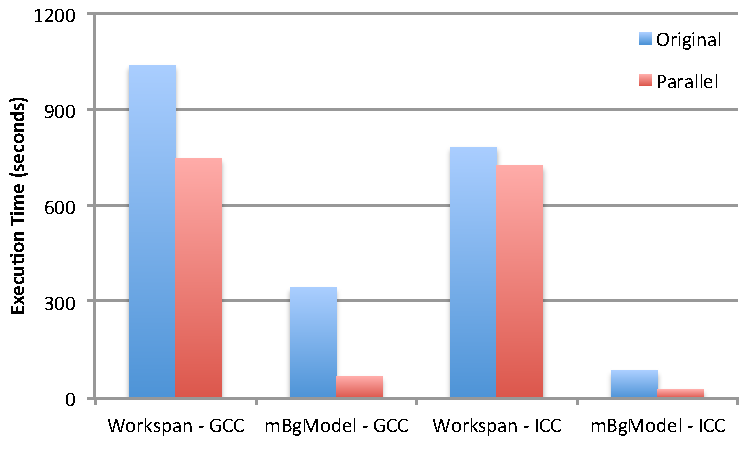
\includegraphics[height=4cm]{fig02}
\vspace{-5pt}
\caption{Impact of Parallelization on Workflow Performance}
\vspace{-10pt}
\label{fig:parallel}
\end{figure}


Now we compare the impact of cluster configurations on the performance of Montage workflow. As shown in Table \ref{tbl:cluster}, four different clustering configurations are being tested.  Cluster M3.2X uses the m3.2xlarge instances from the M3 general purpose product family, while clusters C3.2X, C3.4X and C3.8X uses instances from the C3 compute optimized product family. All these clusters have the same number of total vCPUs. The difference lies in the size of the worker node and the number of worker nodes in the cluster.


\begin{figure}[t!]
\centering
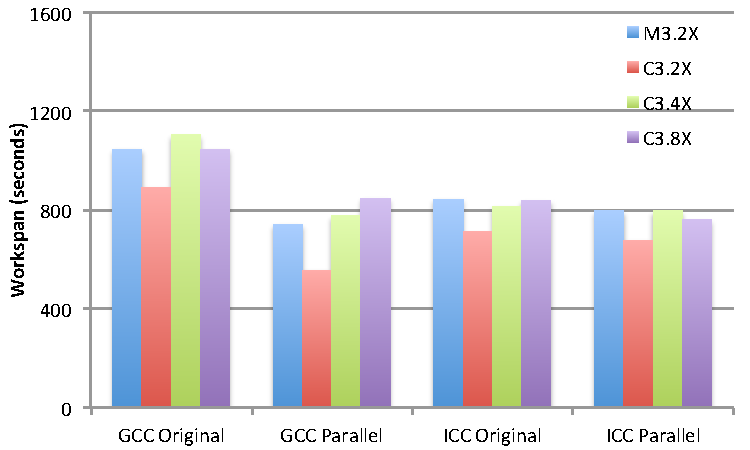
\includegraphics[width=6cm]{fig03}
\caption{Impact of Cluster Configuration - Makespan}
\label{fig:cluster}
\end{figure}

\begin{figure}[t!]
\centering
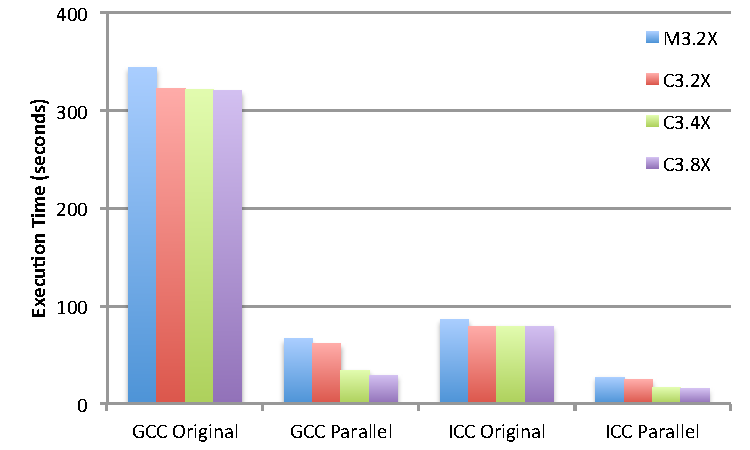
\includegraphics[width=6cm]{fig04}
\caption{Impact of Cluster Configuration - mBgModel}
\label{fig:mBgModel}
\end{figure}

\begin{figure}[t!]
\centering
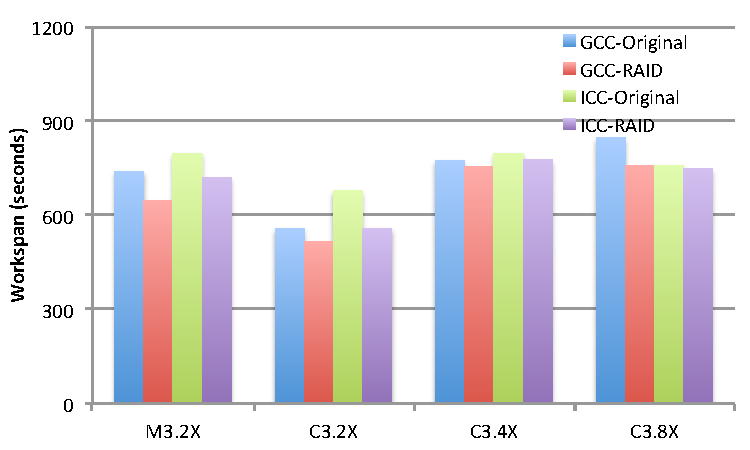
\includegraphics[width=6cm]{fig05}
\caption{Impact of RAID 0 on Makespan}
\label{fig:raid}
\end{figure}

\begin{figure}[t!]
\centering
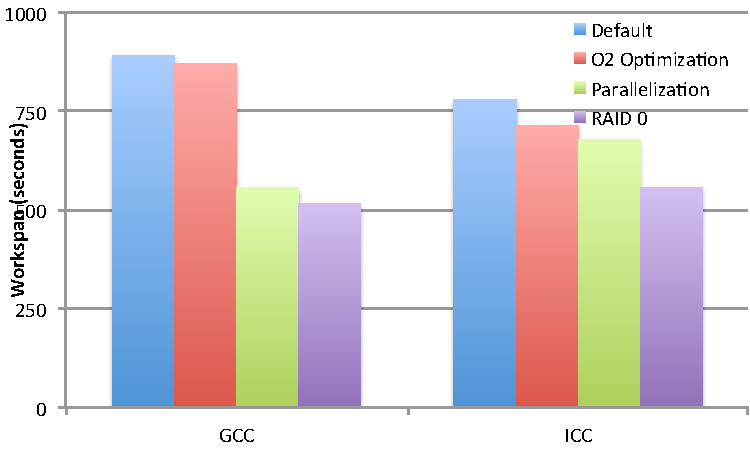
\includegraphics[width=6cm]{fig06}
\caption{Combination of Optimization Techniques}
\label{fig:combine}
\end{figure}

Figure \ref{fig:cluster} shows the impact of cluster configuration on the makespan of the 6.0 degree Montage workflow. In general, the C3.2X cluster has better performance than the other clusters. Figure \ref{fig:mBgModel} show the impact of cluster configuration on the execution time of task mBgModel. With the original version, the execution time of task mBgModel is the same for each VM type with a particular compiler. With the parallelized version, the execution time of mBgModel decreases as the number of vCPUs on the worker node increases. Such reduction in execution time is significant between C3.2X and C3.4X clusters, but is insignificant between C3.4X and C3.8X clusters. 

In order to understand the above-mentioned performance difference, we monitor the CPU and disk utilization status during the test runs. We find out that on average the CPU utilization rate is about 20 to 30 percent during the test runs, while disk utilization is about 80 to 90 percent most of the time. Considering the fact that a 6.0 degree Montage workflow produces 22,850 intermediate files during its execution, we can determine that the Montage workflow is disk I/O intensive, and disk I/O presents a bottleneck in the execution. Such a hypothesis can be verified by the resource consumption pattern as shown in Figure \ref{fig:pattern}. In order to improve disk I/O capability, we create a RAID 0 configuration using the two SSD disk available on the instances, and setup EXT3 file system on the RAID device for data storage. The binaries are compiled with the -O2 flag, and the parallelized version of mBgModel is used for the testing. As shown in Figure \ref{fig:raid}, RAID 0 further reduces the makespan for all test runs. Among all test runs, binaries compiled with GCC running on C3.2X clusters has the shortest makespan.

Apart for the demand for CPU resources, the Montage workflow is at the same time I/O intensive in that a large amount of intermediate files are created during the computation. Therefore, improving I/O performance might also be able to speed up the execution. All the VM instances being used in this research have two ephemeral SSD disks, which can be combined using redundant array of independent disks (RAID) technology for data redundancy or performance improvement. In this research, we use RAID 0  to improve I/O performance through parallelism of read and write operations across multiple disks. Figure \ref{fig:raid} shows the impact of RAID 0 on the makespan of the 6.0 degree Montage workflow. On all clusters, RAID 0 introduces various degree of performance improvement, but the performance improvement is more significant for clusters M3.2X and C3.2X.

Figure \ref{fig:combine} shows the combined effect of the above-mentioned optimization techniques. In this example, a 6.0 degree Montage workflow runs on a C3.2X cluster. For binaries compiled with GCC, the makespan can be reduced from 892 seconds to 517 seconds, representing 42\% makespan reduction. For binaries compiled with ICC, the makespan can be reduced from 779 to 558 secs, representing 28\% makespan reduction. 

\begin{table}[t!]
\caption{Different Cluster Configurations}
\label{tbl:cluster}
\centering
\begin{tabular}{|p{3.0cm}|p{3.0cm}|p{3.0cm}|p{3.0cm}|p{3.0cm}|}
\hline
Config & M3.2X & C3.2X & C3.4X& C3.8X\\ \hline
VM Type & m3.2Xlarge & c3.2Xlarge & c3.4Xlarge& c3.8Xlarge\\ \hline
VM vCPU & 8 & 8 & 16 & 32 \\ \hline
VM MEM & 30 GB & 15 GB & 30 GB & 60 GB \\ \hline
VM DISK & 2 X 80 GB & 2 X 80 GB & 2 X 160 GB & 2 X 320 GB \\ \hline
VM Price & 0.56 USD & 0.42 USD & 0.84 USD & 1.68 USD \\ \hline
Total Nodes & 4 & 4 & 2 & 1 \\ \hline
Total vCPU & 32 & 32 & 32 & 32 \\ \hline
Total Cost & 2.24 USD & 1.68 USD & 1.68 USD& 1.68 USD\\ \hline
\end{tabular}
\end{table}


\section{Summary}
\label{v1_sec:summary}

In this chapter, we use various techniques to optimize the execution of a 6.0 degree Montage workflow running on Amazon EC2. We find out that 

\begin{itemize}
	\item Compiler optimization can be used as general approach to optimize the execution of a scientific workflow. Workflow visualization techniques can be used to generate the resource consumption pattern, as well as identify the bottleneck of a workflow. The bottleneck identified can be further optimized with code level parallelization techniques. The results show that parallelism is the primary source of performance gain in modern computing systems.

    \item On Amazon EC2, further makespan reduction can be achieved by using different cluster configurations without impact on cost. Since Montage workflows are also I/O intensive, additional performance gain can be achieved using RAID 0, which improves I/O performance through parallelism of read/write operations.

\end{itemize}



\chapter{Executing Large Scale Workflow Ensembles in Public Clouds}
\label{chapter:dewe_v2}

\section{Introduction}
\label{sec:intro}

Many applications in science and engineering are increasingly formed as workflows with many precedence-constrained jobs, e.g., Montage \cite{montage, web:montage}, LIGO \cite{ligo}, and CyberShake \cite{cybershake}. Scientists need to run these workflows with different parameters repeatedly, or use a combination of different workflows to achieve an ultimate goal. We use the term \textbf{workflow ensemble} to represent an entire scientific analysis as a set of interrelated but independent workflow applications. In modern scientific computing applications, a single scientific workflow often becomes very large in terms of the number of constituting jobs and input data size, which is already a challenge in terms of resource provisioning and scheduling. The situation is further complicated by the number of interrelated but independent workflows in a workflow ensemble. Thus, the efficient execution of a workflow ensemble with multiple workflows is of great practical importance.

Most researchers in the scientific workflow community use existing workflow management systems that were designed with grid as the target execution environment. In a grid environment, the computing resources are considered as heterogeneous. It is necessary to schedule critical jobs to worker nodes with more processing power, and to avoid large data transfer over connections with small bandwidth. In public clouds, a homogeneous environment can be created by launching instances with the same instance type in the same availability zone. This brings new opportunities in optimizing execution coordination, which was not considered in existing workflow management systems. From a cost perspective, most service providers charge computing resources in an hourly manner, where partial hour usage is charged as a full hour. For example, a particular workflow takes 61 minutes to execute on a 10-node cluster, but can be completed in 59 minutes on a 11-node cluster. The cost to run the workflow on a 10-node cluster is 20 instance hours, but would be only 11 instance hours on a 11-node cluster. For large scale workflow ensembles, it is critical that the execution can be completed within both cost and deadline constrains. There have been some previous studies on these two aspects. However, existing literature only provides small scale results or uses simulations instead of real scientific applications.


\begin{figure*}[ht]
\centering
\fbox{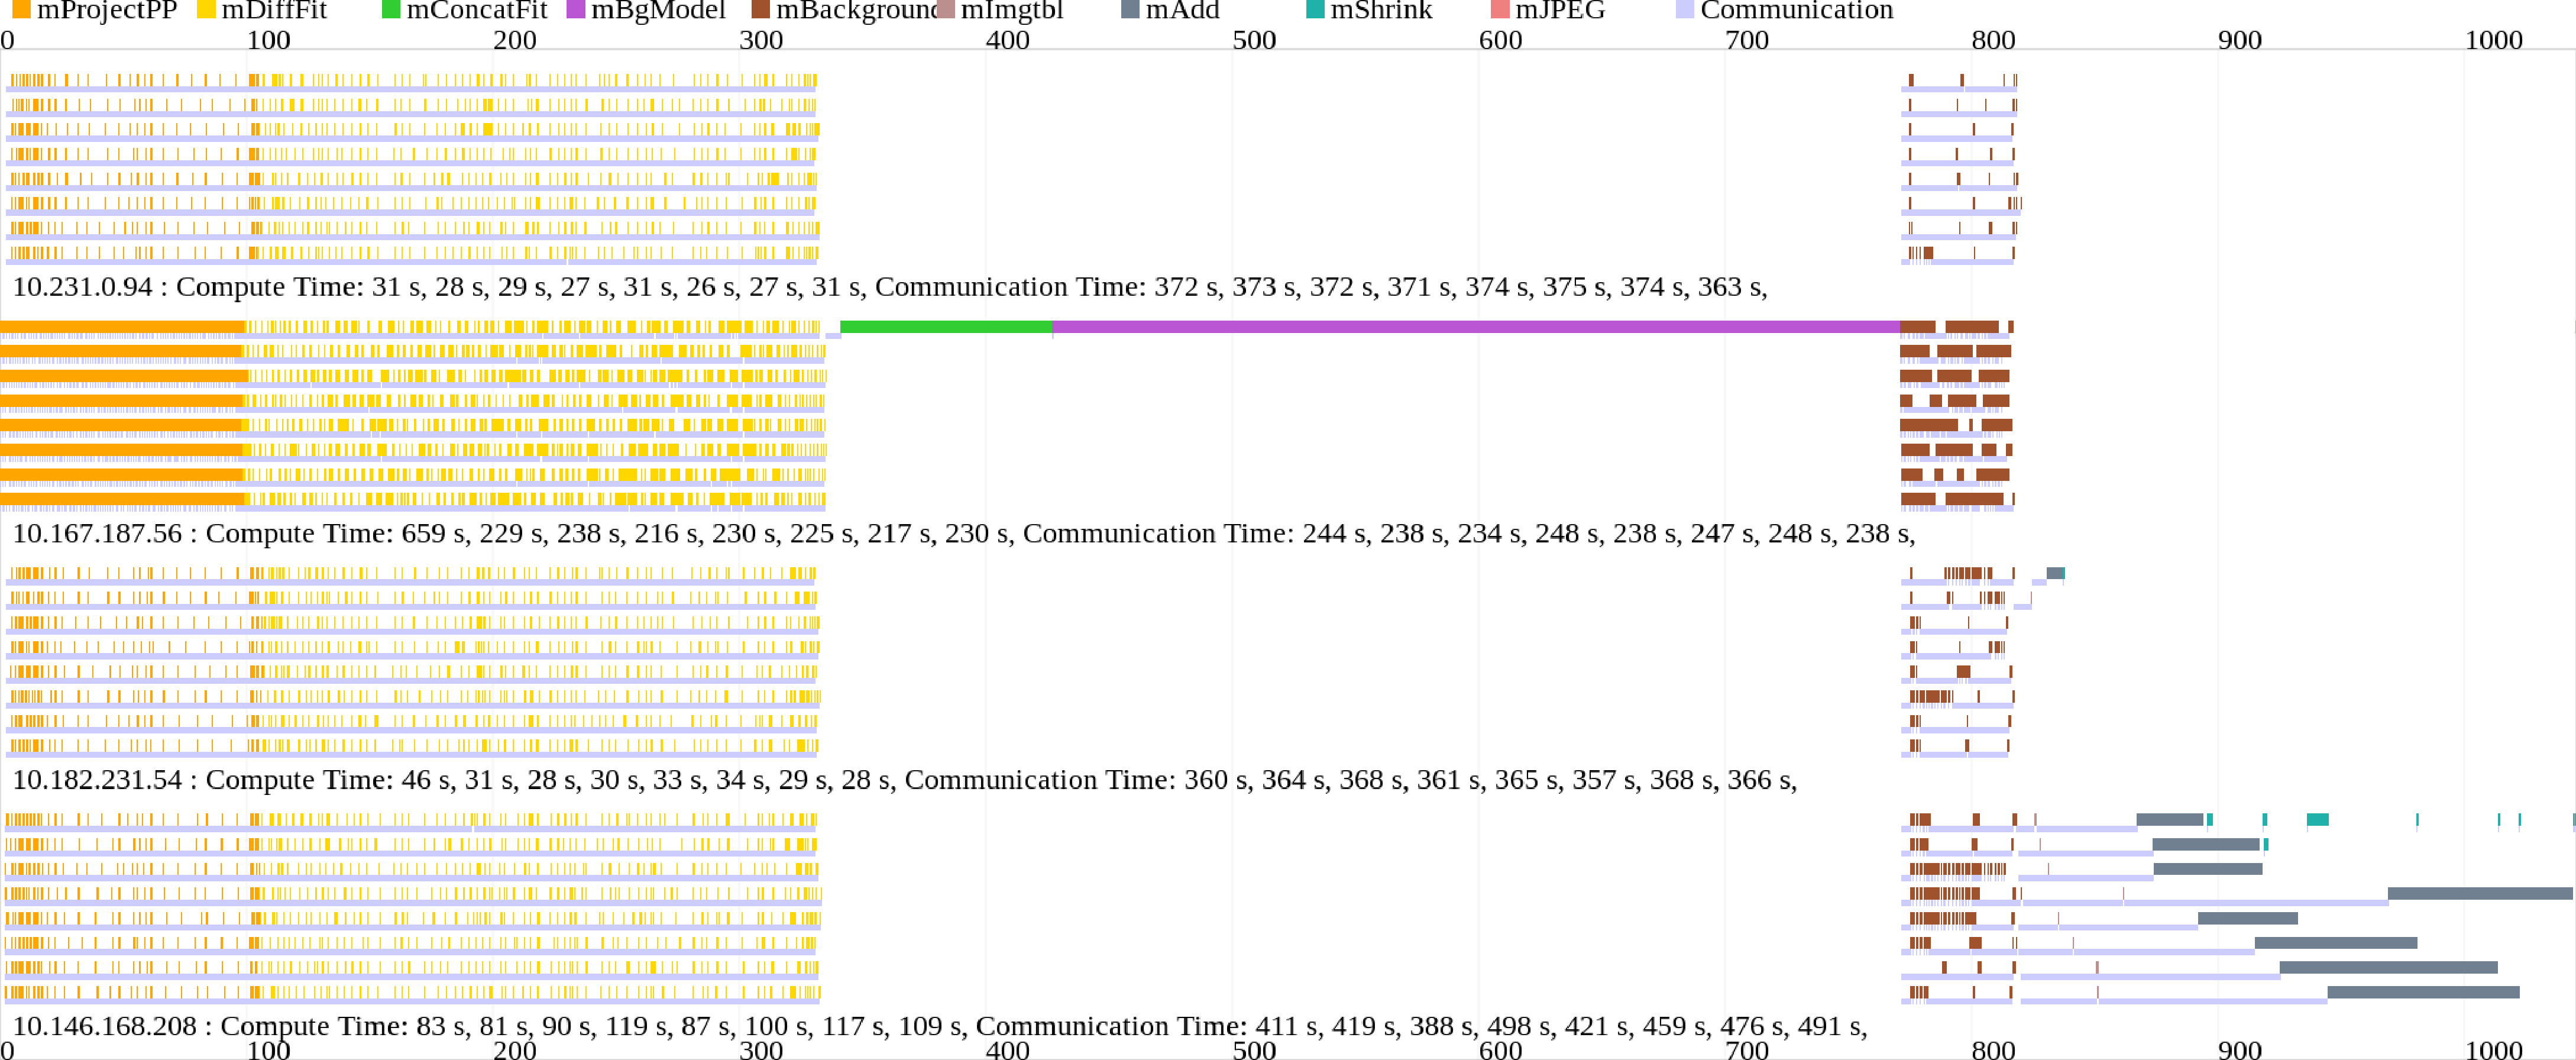
\includegraphics[width=16cm]{montage_visualization}}
\caption{Detailed visualization of a 6.0 degree Montage workflow running 4 m3.2xlarge instaces using DEWE v1. Each worker node has 8 vCPU, 30 GB of memory, and 2 x 80 GB SSD storage. The horizontal axis represents time in seconds, while the vertical axis represents vCPU slots in the cluster. Each vCPU is represented by two horizontal bars, with job execution activities on the first horizontal bar and data staging activities on the second horizontal bar. For each worker node, the graph shows the IP address of the worker node, the time spent on job execution (compute time) and the time spent on data staging (communication time) for each vCPU slot. As shown in the graph, the Montage has a clear three-stage pattern, with significant resource utilization in the second and third stage.}
\label{fig:montage_visualization}
\end{figure*}

In this chapter, we choose Montage as a representative example of large scale scientific workflows for our case study due to the following reasons:  (1) there are a large number of small jobs that can run in parallel, (2) scientists in astronomy do have the need to execute Montage workflow ensembles; for example, a set of small image mosaics are needed to produce a large image mosaic (the Galactic Plane workflow ensemble \cite{deelman2013hosted} consists of 17 workflows, each of which contains 900 sub-workflows), (3) Montage workflows are data-intensive, and (4) The Montage source code and data is available to the general public (i.e., open source). (1) is closely related to execution coordination, (2) presents challenges in resource provisioning, and (3) is closely related to data staging. Therefore, Montage is an ideal example that enables us to study these three challenges in executing large scale workflow ensembles in public clouds.

Montage is an astronomical image mosaic engine that assembles individual images of the sky into a mosaic. A 6.0 degree Montage workflow creates a 6-by-6 degree square mosaic centered at a particular region of the sky (e.g., M16). The number of jobs and input data files increases with the number of degrees of the mosaic. A 6.0 degree Montage workflow contains 8,586 jobs, 1,444 input files with a total size of 4.0 GB, and 22,850 intermediate files with a total size of 35 GB. In practice, a set of smaller image mosaics are needed to produce a large image mosaic, where each smaller image mosaic is generated by a Montage workflow. For example, the Galaetic Plane workflow ensemble \cite{deelman2013hosted} consists of 17 workflows, each of which further contains 900 sub-workflows. 


The structure of the Montage workflow has been fully explored in the previous chapter. The progress of the workflow has a three-stage pattern. During the first stage, a large number of mProjectPP jobs run in parallel, followed by a large number of mDiffFit jobs running in parallel. During the second stage, two jobs mConcatFit and mBgModel run one after another, during which no other jobs are eligible to run. In this paper, we consider mConcatFit and mBgModel as blocking jobs because they block the execution of other jobs. During the third stage, a large number of mBackground jobs run in parallel, followed by a small number of mImgTbl, mAdd, mShrink, and mJPEG jobs.

As shown in Figure  \ref{fig:montage_visualization}, the mProjectPP, mDiffFit and mBackground jobs are small jobs with very short execution time within the range of a few seconds. However, they consume and produce a large number of intermediate data files. Staging these intermediate data files between worker nodes causes significant communication cost. Considering the large number of such jobs, it is desirable to have more worker nodes to speed up the execution. However, the communication costs increases when the number of worker nodes increases, resulting in clustering performance degradation. Furthermore, the execution time of the second stage is approximately 40\% of the makespan. During this stage, among all the available computing resources only one CPU core is being utilized. When the cluster is larger, more computing resources are being wasted during this stage. In a Montage workflow ensemble, resource under-utilization can be worse due to the lack of coordination between individual sub-workflows. Therefore, the Montage workflow ensemble represents a scheduling dilemma requiring trade-offs between cost and performance. 

In this chapter, we address two main challenges in realizing benefits of using public clouds when executing large-scale workflow ensembles with both deadline and cost constrains: (1) execution coordination, and (2) resource provisioning. To this end, we develop DEWE v2 \footnote{The source code is available from \url{https://github.com/qyjohn/DEWE.v2}.}, a major overhaul of our preliminary version of DEWE \cite{dewev1}. DEWE v2 is a pulling-based workflow execution system that is capable of executing large scale scientific workflow ensembles in public clouds. Using DEWE v2, we address the above-mentioned challenges in executing large-scale workflow ensembles in public clouds. The specific contributions of this paper are:


\begin{itemize}
  \item We demonstrate that the pulling approach has better performance over the scheduling approach in executing large scale scientific workflow ensembles in public clouds. 
  \item We demonstrate that incremental job submission can effective shape the resource utilization pattern, thus achieve better resource utilization than batch job submission. 
  \item We propose a two-step strategy to provision computing resources in public clouds for executing large scale scientific workflow ensembles to meet both cost and deadline constraints. 
\end{itemize}

We have extensively evaluated DEWE v2 using Montage workflow ensembles with varying sizes and different configurations of EC2 clusters. In particularly, our large-scale experiments were conducted using up to 200 6.0 degree Montage workflows containing over 1.7M jobs and dealing with approximately 7 TB of data; and, four Amazon EC2 clusters with different instance types (\emph{c3.8xlarge, r3.8xlarge and i2.8xlarge}, which are the largest instances in their instance families) were set up consisting of up to 1,280 vCPUs. 

The rest of this chapter is organized as follows. In Section \ref{v2_sec:dewe_v2_design}, we describe the design philosophy, system architecture, and the implementation of DEWE v2. In Section \ref{v2_sec:setup}, we describe our experiment environment in details, including the benchmark results of the EC2 instances being used in the experiments. In Section \ref{v2_sec:dewe_v2_performance}, we evaluate the performance of DEWE v2, using Pegasus as a comparison. We also compare the the efficiency of batch submission and incremental submission, as will as the robustness of DEWE v2. In Section \ref{v2_sec:provision}, we propose a two-step strategy to provision computing resources in public clouds for executing large scale scientific workflow ensembles with both cost and deadline constraints. We demonstrate the effectiveness of the proposed resource provisioning strategy with its incorporation into DEWE v2. In Section \ref{v2_sec:disk_io}, we compare the disk I/O performance of EC2 clusters with the disk I/O performance observed on supercomputers in the literature. We present a summary of the content in this chapter in Section \ref{v2_sec:summary}.


\section{Design and Implementation of DEWE v2}
\label{v2_sec:dewe_v2_design}

DEWE v2 is an improved version of DEWE, a lightweight framework for distributed elastic workflow execution developed at the University of Sydney. In subsequent sections, we call the original version DEWE v1.  DEWE v2 shares some fundamental design concepts with DEWE v1; hence the name. With DEWE v1, researchers can only execute one workflow at a time. DEWE v2 is capable of executing a large number of workflows in parallel, hence the ability to execute large-scale workflow ensembles. DEWE v1 was developed in Python, and DEWE v2 was developed in Java to reduce third-party package dependencies. 

In this section, we describe the design philosophy, system architecture, as well as the implementation of DEWE v2. 


\subsection{Design Philosophy}
\label{sec:subsec:design_philosophy}


In general, there are two approaches to design and implement a workflow management system. The first approach emphasizes scheduling where the master node maintains the state of all participating worker nodes, assigns jobs to worker nodes using various resource scheduling algorithms, as well as stages necessary data files to the worker nodes for job execution. The second approach emphasizes a stateless design where the master node publishes all pending jobs to a queue, and a number of un-managed worker nodes pull the job queue and compete for jobs to execute. Most existing workflow management systems adopt the scheduling approach, including Condor DAGMan, Pegasus, and Kepler. 

In a grid environment, the computing resources are considered as heterogeneous. It is necessary to schedule critical jobs to worker nodes with more processing power, and to avoid large data transfer over connections with small bandwidth. Furthermore, data transfer between worker nodes is usually accomplish with file transfer tools such as FTP, SFTP, GridFTP, or SCP. In the workflow community, the cost to stage the output of one job to the node that will run the second job is defined as communication cost. An important assumption with the scheduling approach is the communication cost is none-zero value when both jobs are running on two different nodes, but becomes zero when the two jobs are running on the same node because no data transfer is needed. Therefore, a good scheduling algorithm should always try to minimize data transfers. With the scheduling approach, the scheduling overhead can be overcome by utilizing the computing resources in a more efficient way, resulting in shorter makespan. 

With Amazon EC2, a homogeneous environment can be achieved by launching all the worker nodes with the same instance type in the same placement group. For critical jobs, the computation cost remains the same regardless of the worker node they run on. Furthermore, data transfer between worker nodes can be replaced with a shared file system such as NFS. With a large scale workflow ensemble, the number and size of the input files overwhelm the memory available on the worker nodes. The result is the communication cost becomes the time needed to read the input files from the shared file system, which is the same regardless of the worker node. In this case, the pulling approach has advantages over the scheduling approach because it avoids the scheduling overhead.


\subsection{System Architecture}
\label{sec:subsec:system_architecture}

\begin{figure}[!t]
	\centering
	\hspace{-5pt}
	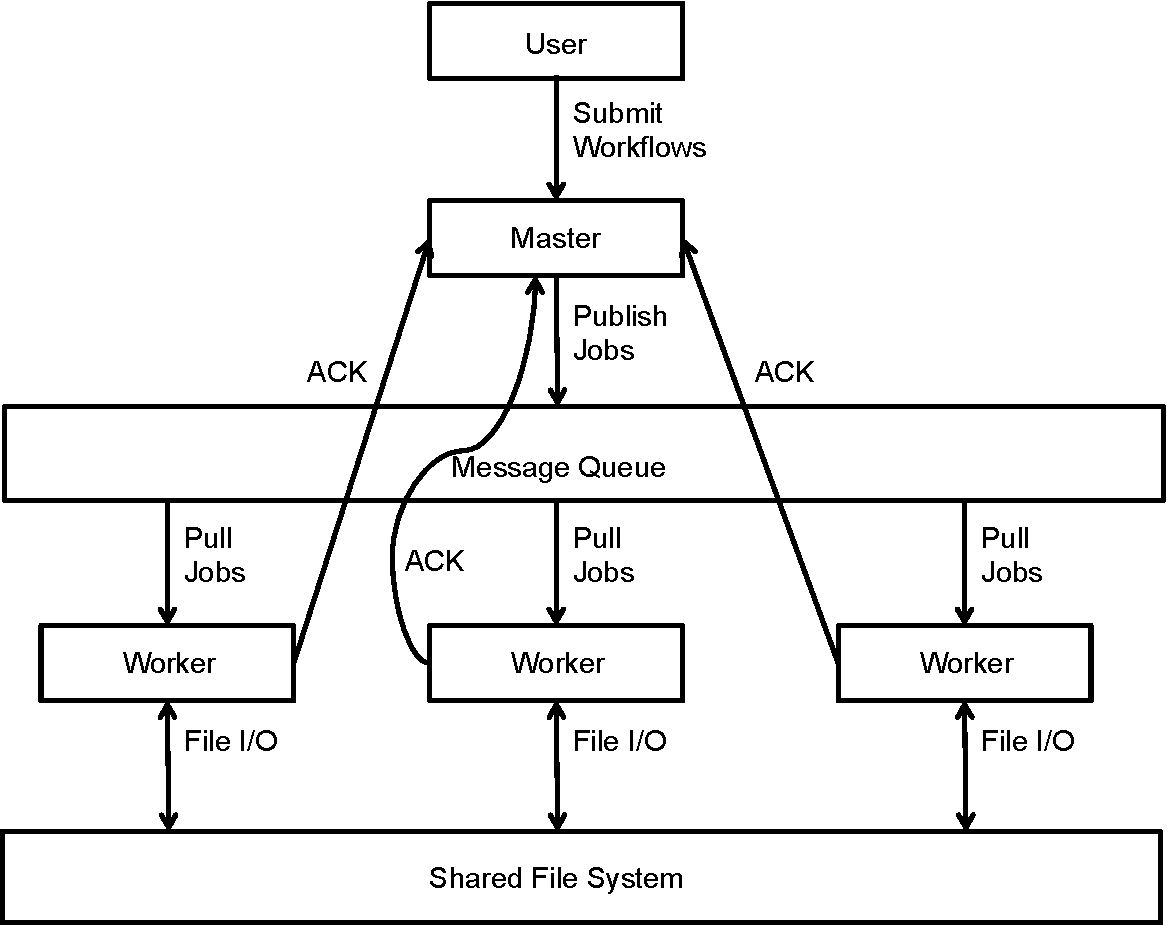
\includegraphics[width=7cm]{dewe_v2_architecture}
    \vspace{5pt}
	\caption{The architecture of DEWE v2.}
	\label{fig:dewe_v2_architecture}
\end{figure}


Both DEWE v1 and DEWE v2 are pulling based workflow execution engines, with a master node managing a message queue and multiple worker nodes pulling the message queue for jobs to execute. With DEWE v1, the master node also manages the input and output files. When a worker node pulls a job for execution, it queries the master node for the location of the input files, transfers the input files from the worker nodes that have/produce those files, executes the job and reports the results back to the master node. DEWE v2 removes this scheduling layer by utilizing a POSIX-compliant shared file system, which significantly simplify the architecture design. 



Figure \ref{fig:dewe_v2_architecture} shows the architecture design of DEWE v2. The system includes a master daemon, a worker daemon, and a workflow submission application. In a cluster environment, one of the nodes runs the master demon, which can optionally run the worker daemon at the same time. All other nodes run the worker daemon. Using the workflow submission application, scientists can submit workflows to the master daemon from any nodes at any time. 

The master daemon only manages the progress of the workflow, and publishes jobs that are eligible to run to a message queue. It has no knowledge about the worker nodes, but assumes that the worker nodes are homogeneous in terms of computing capability and communication bandwidth. 

On the basis of ``first come, first served", the worker nodes actively pull the message queue for jobs to execute. When the job is successfully executed, the worker node sends an acknowledge message to the master daemon. Based on the acknowledge messages from the worker nodes, the master daemon publishes new jobs that are eligible to run to the message queue.

A POSIX-compliant shared file system is used to facilitate the data sharing between worker nodes. When an output file is generated by a job on a worker node, it is immediately accessible from other worker nodes and can be used as inputs files for other jobs. This shared file system can be provided by either a centralized storage server (such as a NAS device) or a distributed storage system (such as GlusterFS). We assume that all worker nodes have equal access to the shared file system. A workflow is encapsulated in a folder on the shared file system, including the DAG file, the executable binaries, as well as the input and output files. 

To increase the robustness of the system, a timeout mechanism is added to the DAG management module in the master daemon. A job can have a user-defined timeout value or a system-wide default timeout value. If a job has been checked out from the message queue for execution but the corresponding acknowledgment is not received by the master daemon within the timeout setting, the master daemon publishes the job to the message queue again. With this timeout approach, any worker node can fail at any time and the failed jobs will be automatically resubmitted to the message queue for execution by other worker nodes when the timeout occurs.

The master daemon is capable of managing multiple workflows concurrently. When precedence dependencies are met, jobs in different workflows are published to the same message queue for execution. Therefore, multiple workflows can be executed in parallel on the same cluster. 

As we can see, DEWE v2 significantly simplifies the workflow execution process. There is no scheduling at any stage during the execution of the workflow. The stateless design of the worker node allows the cluster to scale in or scale out according to the actual workload requirements. 



\subsection{Implementation of the Master Daemon}
\label{sec:subsec:master_daemon}

At the core of DEWE v2 is a message queue system based on RabbitMQ. We use three separate topics in the message queue for workflow submission, job dispatching, and job acknowledgment. When the workflow submission application submits a workflow, meta data about the workflow (the name of the workflow, as well as the path to the related folder on the shared file system) is published to the workflow submission topic. The master daemon pulls meta data about the workflow from the workflow submission topic, then parses the DAG file and stores the job dependencies information into a data structure. If a job has no pending dependency precedence requirements, the master daemon publishes meta data about the job (the location of the binary executable with input and output parameters) to the job dispatching topic.

When a job is checked out by a worker node for execution, the worker nodes sends a message to the job acknowledgment topic indicating the job is now running. When a job is successfully executed on a worker node, the worker node sends another message to the job acknowledgment topic indicating the job is now completed. The master daemon pulls the job acknowledgment topic for such messages. If the message indicates a job is running, the master daemon marks the job as "running" so that the job is no longer visible to other worker nodes. If the message indicates a job is completed, the master daemon marks the job as "completed" and updates the status of all pending jobs that depend on the completed job. When a job has no pending precedence requirements it becomes eligible to run. Then the master daemon publishes meta data about jobs that are eligible to run to the job dispatching topic, where they are pulled by the worker nodes for execution.

The master daemon periodically examines the execution status of all "running" jobs. If a job is checked out by a worker node for execution but the corresponding acknowledgment indicating the job is completed is not received within its timeout setting, a timeout event is triggered. The master daemon then resubmits meta data about the job to the job dispatching topic so that other worker nodes can execute the job again.


\subsection{Implementation of the Worker Daemon}
\label{sec:subsec:worker_daemon}

The worker daemon has a stateless design. The only knowledge it has about the whole workflow execution system is the address of the message queue. It has no knowledge about the master node, other worker nodes in the system, or the jobs that have been executed on the worker node itself. It reads input files from, and writes output files to, the shared file system, just like using a local file system. Such a stateless design allows the cluster to scale in or scale out according to the actual workload requirements. 

The worker daemon pulls the job dispatching topic for jobs to execute. Upon receiving a job from the message queue, the worker daemon sends a message to the job acknowledgment topic indicating the job is now running. A separate thread is launched by the worker daemon to handle each individual job. Upon completion of the job, the worker daemon sends another message to the job acknowledgment topic indicating the job is now completed. The thread associated with a job is terminated when the job is completed. 

To avoid resource competition among concurrently running jobs, we put an upper limit on the number of concurrent job execution threads. The worker daemon stops pulling the job dispatching topic when the number of concurrent job execution threads equals to the number of CPUs available on the worker node. However, the worker daemon does not bind a job to a particular CPU. If a job is implemented in a way that can leverage multiple CPUs (for example,  OpenMP) the desired behavior is preserved. This feature can significant speed up the execution of a workflow when the blocking jobs (such as mConcatFit and mBgModel) are implemented as parallel code. 

\subsection{Implementation of the Workflow Submission Application}
\label{sec:subsec:submission_application}

The workflow submission application accepts two parameters from the user - the name of the workflow, and the path to the related folder on the shared file system. The workflow submission application publishes this information to the workflow submission topic in the message queue system, where it is checked out by the master daemon for further processing. 




\section{Experiment Environment}
\label{v2_sec:setup}

\subsection{Selection of EC2 Instances}
\label{sec:subsec:ec2_selection}


\begin{table}[t!]
\caption{EC2 Instance Types}
\label{tbl:instance_type}
\centering
\begin{tabular}{|p{2.5cm}|p{1.5cm}|p{1.5cm}|p{1.5cm}|p{1.5cm}|p{2.5cm}|}
\hline
Model & vCPU & Memory (GB) & Storage (GB) & Network (Gbps) & Hourly Price  (USD)\\ \hline
c3.8xlarge & 32 & 60  & 2 x 320 & 10 & 1.68\\ \hline
r3.8xlarge & 32 & 244 & 2 x 320 & 10 & 2.80\\ \hline
i2.8xlarge & 32 & 244 & 8 x 800 & 10 & 6.82\\ \hline
\end{tabular}
\end{table}



\begin{table}[t!]
\caption{Disk I/O Capacity of EC2 Instance Types}
\label{tbl:instance_disk_io}
\centering
\begin{tabular}{|p{2.5cm}|p{2.5cm}|p{2.5cm}|p{2.5cm}|p{2.5cm}|}
\hline
Model & Sequential Read (MB/s) & Sequential Write (MB/s) & Random Read (MB/s)& Random Write (MB/s)\\ \hline
c3.8xlarge & 250 & 800  & 400 & 600 \\ \hline
r3.8xlarge & 350 & 1000 & 700 & 800 \\ \hline
i2.8xlarge & 2200 & 3800 & 1800 & 3600 \\ \hline
\end{tabular}
\end{table}



Amazon Web Services (AWS) are widely recognized as examples of public cloud services. Over the past years, the market witnessed a trend in developing new applications on AWS, or migrating existing applications to AWS. In this paper, all the experiments are carried out on AWS Elastic Computer Cloud (EC2) in its us-east-1 (N. Virginia) region. AWS EC2 provides a wide range of instance types for different use cases. Different instance types have different combinations of vCPU, memory, storage, and networking capacity. We use the c3.8xlarge, r3.8xlarge, and i2.8xlarge instance types for our experiments. With AWS EC2, c3.8xlarge is the largest instance type for compute intensive applications, r3.8xlarge is the largest instance type for memory intensive applications, and i2.8xlarge is the largest instance type for storage intensive applications. Table \ref{tbl:instance_type} lists the specifications of the selected instance types. Apart from the properties listed in Table \ref{tbl:instance_type}, c3.8xlarge instance type uses Intel Xeon E5-2680 v2 (Ivy Bridge) processors, while r3.8xlarge and i2.8xlarge instance types use Intel Xeon E5-2670 v2 (Ivy Bridge) processors.  

On all of the selected instance types, the storage devices are SSD-backed instance store volumes (storage from disks that are physically attached to the host computer). To achieve the best disk I/O performance, we combine all the instance store volumes available on the instance using redundant array of independent disks (RAID) technology in a RAID 0 configuration. All the workflow related disk I/O operations are configured to occur on the RAID device. The file system being used on all worker nodes is ext4.

\subsection{Benchmark of EC2 Instances}
\label{sec:subsec:ec2_benchmark}

\begin{figure*}[t!]
\centering
\vspace{-10pt}
 \subfloat[CPU Benchmark]{ 
    \label{fig:subfig:benchmark_cpu}  
    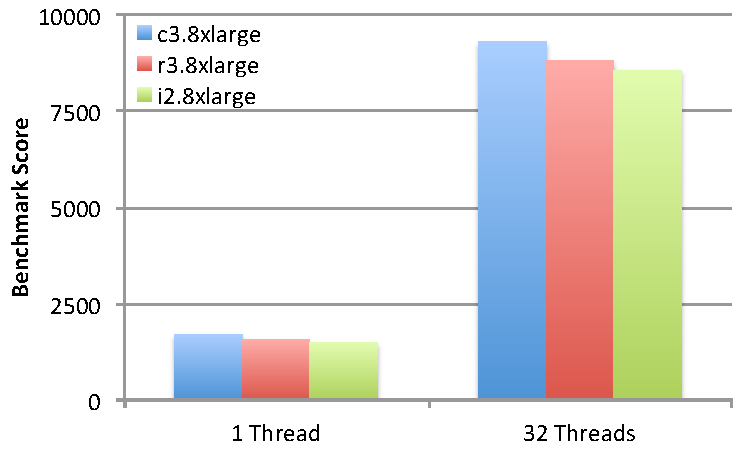
\includegraphics[width=6cm]{benchmark_cpu}} 
 \hspace{5pt}
 \subfloat[Memory Benchmark]{ 
    \label{fig:subfig:benchmark_mem}  
    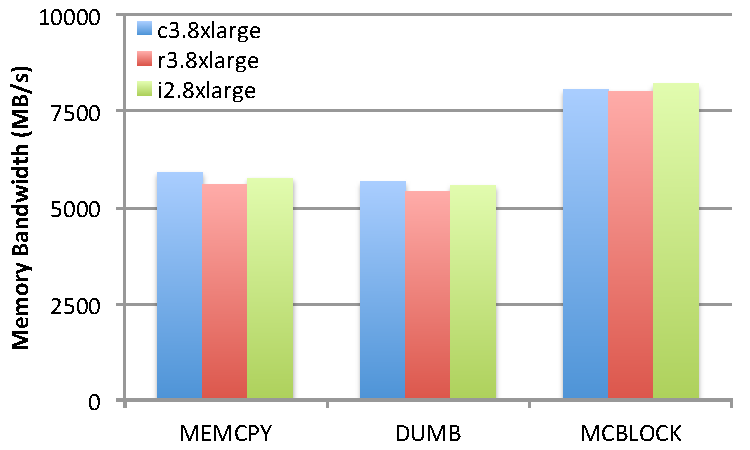
\includegraphics[width=6cm]{benchmark_mem}} 
  \hspace{5pt}
 \subfloat[Disk IO Benchmark]{ 
    \label{fig:subfig:benchmark_disk}  
    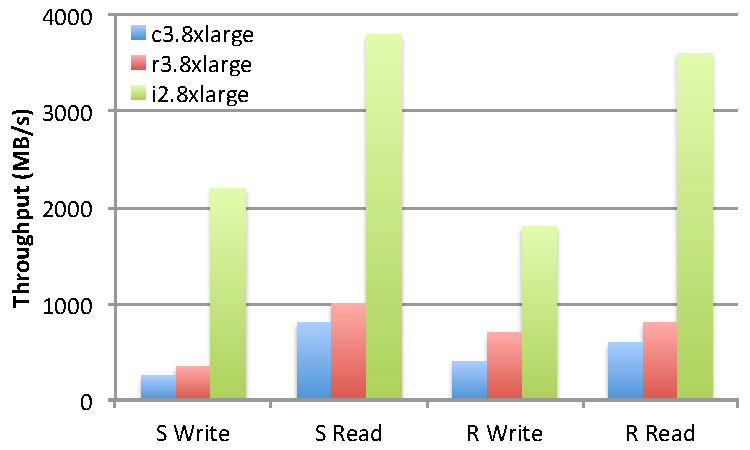
\includegraphics[width=6cm]{benchmark_disk}} 
  \caption{Benchmark of CPU, memory and disk IO for c3.8xlarge, r3.8xlarge and i2.8xlarge instances.} 
  \label{fig:instance_benchmark} 
\end{figure*}


Many people perceive computing resources on AWS as of equal performance across instance types. For example, one vCPU on c3.8xlarge instances is expected to have the same performance as one vCPU on r3.8xlarge instances; the SSD storage on c3.8xlarge instances is expected to have the same performance as the SSD storage on r3.8xlarge instances. We use UnixBench \footnote{The source code is available from \url{http://code.google.com/p/byte-unixbench/}.}, MBW \footnote{The man page is available from \url{http://manpages.ubuntu.com/manpages/karmic/man1/mbw.1.html}.}, and IOZone \footnote{The source code is available from \url{http://www.iozone.org}.} to benchmark the CPU, memory and disk IO performance of the three instance types being used in this study. 

UnixBench is a benchmark suite that can be used to evaluate the overall performance of Unix-like systems. The original version of UnixBench was developed in 1983 at Monash University. Afterwards it was updated and revised by many people over the years. In this study we used the version ``byte-unixbench'' available from the Google Code website. In the UnixBench benchmark suite, several different tests are carried out to evaluate the performance of the system. Based on the scores of the above-mentioned different tests, a system level score (System Benchmarks Index Score) is calculated. In this study, we use this system level score to compare the CPU performance of different VM instances. The test results are presented in Figure \ref{fig:subfig:benchmark_cpu}. In the 1-thread test, all three instance types achieve similar scores. In the 32-thread test, the c3.8xlarge instance achieves the best score, followed by r3.8xlarge and then i2.8xlarge. 

MBW measures available memory bandwidth by copying large arrays of data in memory. In the MEMCPY test, we measure the speed achieved while copying a 128 MB array from one area of memory to another. In the DUMB test, we allocate two arrays of 128 MB, then copy the value of each element in the first array to the corresponding element in the second array with operations such as "b[i] = a[i]". The MCBLOCK test is similar to the MEMCPY test, but the copy operation is carried out in 4096-byte blocks. As shown in Figure \ref{fig:subfig:benchmark_mem}, all three instance types have similar memory performance in all three tests. The r3.8xlarge instance performs slightly worse in all three tests, but the performance difference is insignificant. 

IOZone benchmarks the performance of the underlying file system by generating and measuring a variety of file operations. Different scientific computing applications have different disk IO patterns. In general, applications dealing with large input / output files (such as large scale sorting) demands sequential IO capability, while applications dealing with a large number of small input / output files (such as Montage) demands random IO capability. In the sequential IO test, we use two 256 GB test files as the input to make sure that they will not fit into the memory of the instance being tested. In the random IO test, we use 2,000,000 small files ranging from 4 KB to 40 MB as the input, and the total size of the input files is 512 GB. As shown in Figure \ref{fig:subfig:benchmark_disk}, the disk IO performance is dramatically different for the three instance types. In the sequential write (S Write) test, the sequential write throughput of the RAID0 device on c3.8xlarge instances is only 1/2 of the sequential write throughput of the RAID0 device on r3.8xlarge instances. Since both c3.8xlarge and r3.8xlarge instance types have 2 x 320 GB SSD storage, it is obvious that the SSD disks being used for c3.8xlarge instances are different from the SSD being used for r3.8xlarge instances. The sequential write throughput of the RAID0 device on i2.8xlarge instances is 4 times the sequential write throughput of the RAID0 device on r3.8xlarge instances. Since the i2.8xlarge instance has 8 SSD disks while the r3.8xlarge has 2 SSD disks, it is quite possible that the SSD disks being used for r3.8xlarge and i2.8xlarge instances are the same. Similar trends are also observed in the tests for sequential read (S Rread), random write (R Write), and random read (R Read).


\section{Performance Evaluation of DEWE v2}
\label{v2_sec:dewe_v2_performance}


\subsection{Scheduling vs Pulling}
\label{sec:subsec:scheduling_vs_pulling}


\begin{figure*}[t!]
\centering
\vspace{-10pt}
 \subfloat[Concurrent Threads]{ 
    \label{fig:subfig:dewe2_threads}  
    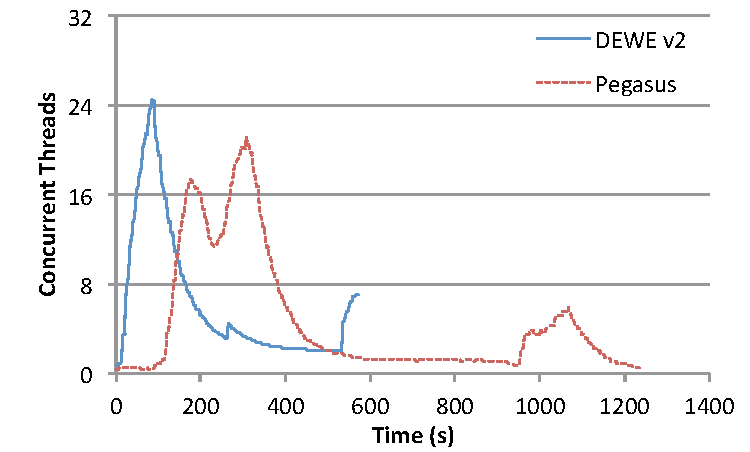
\includegraphics[width=6cm]{compare_threads}} 
 \hspace{5pt}
 \subfloat[CPU Utilization]{ 
    \label{fig:subfig:dewe_v2_cpu}  
    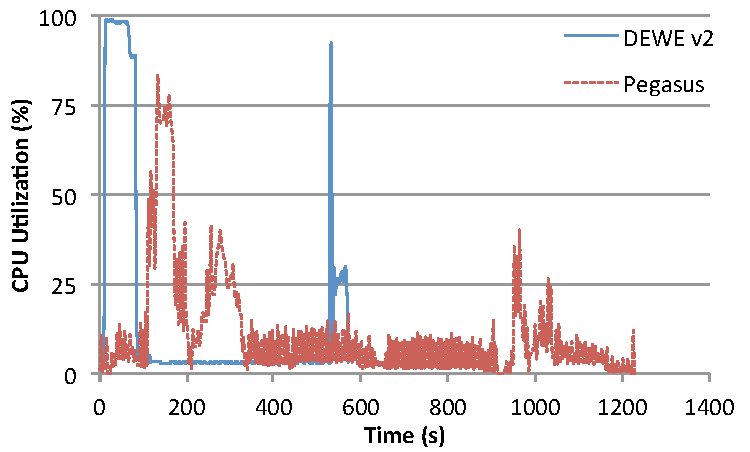
\includegraphics[width=6cm]{compare_cpu}}
 \hspace{5pt}
 \subfloat[Disk Write Operations]{ 
    \label{fig:subfig:dewe_v2_disk_writes}  
    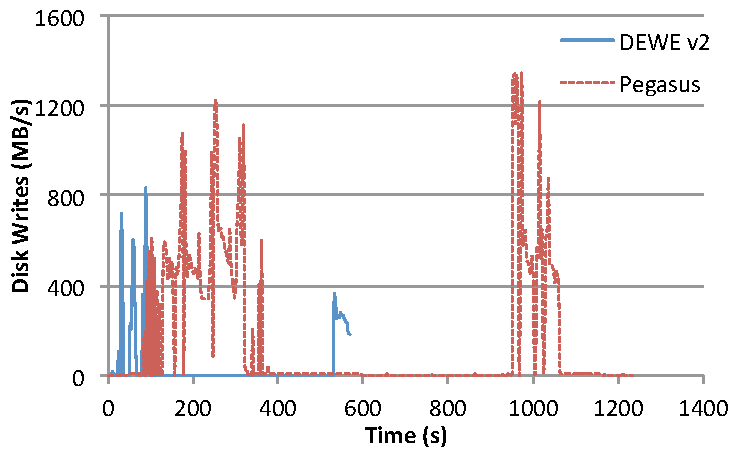
\includegraphics[width=6cm]{compare_disk_writes}} 
  \caption{Resource consumption patterns of one 6.0 degree Montage workflow running on a single-node cluster with DEWE v2 and Pegasus. The instance type being used is c3.8xlarge.} 
  \label{fig:compare_graphs} 
\end{figure*}



\begin{figure*}[t!]
\centering
\vspace{-10pt}
 \subfloat[Total Execution Time]{ 
    \label{fig:subfig:multi_run_makespan}  
    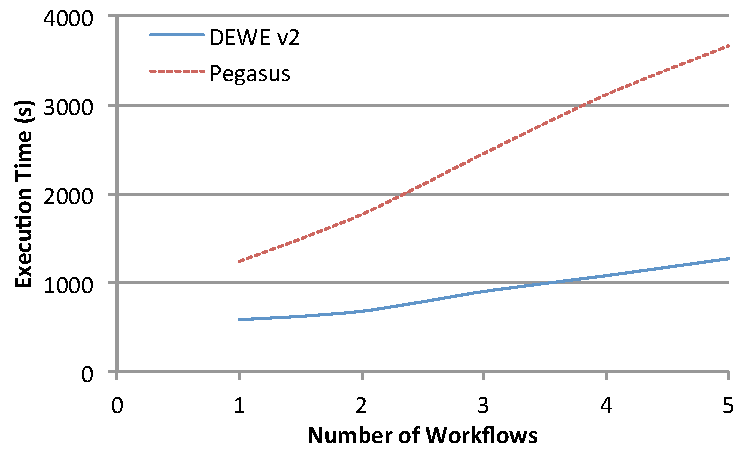
\includegraphics[width=6cm]{multi_run_makespan}} 
 \hspace{5pt}
 \subfloat[Total CPU Time]{ 
    \label{fig:subfig:multi_run_cpu_time}  
    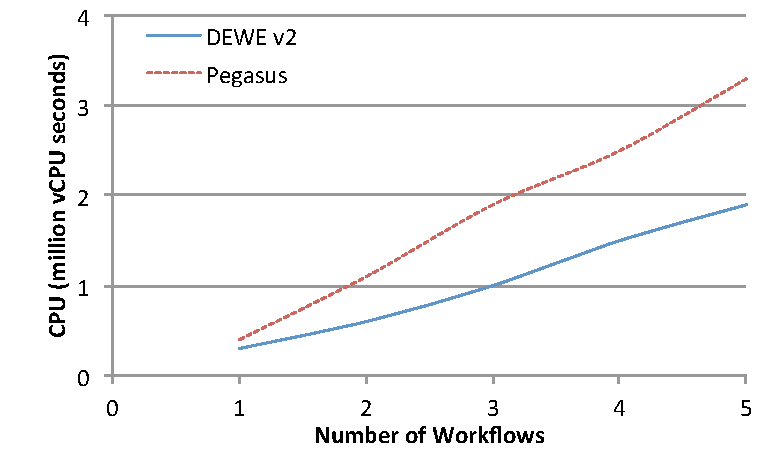
\includegraphics[width=6cm]{multi_run_cpu_time}} 
  \hspace{5pt}
 \subfloat[Total Disk Writes]{ 
    \label{fig:subfig:multi_run_disk_writes}  
    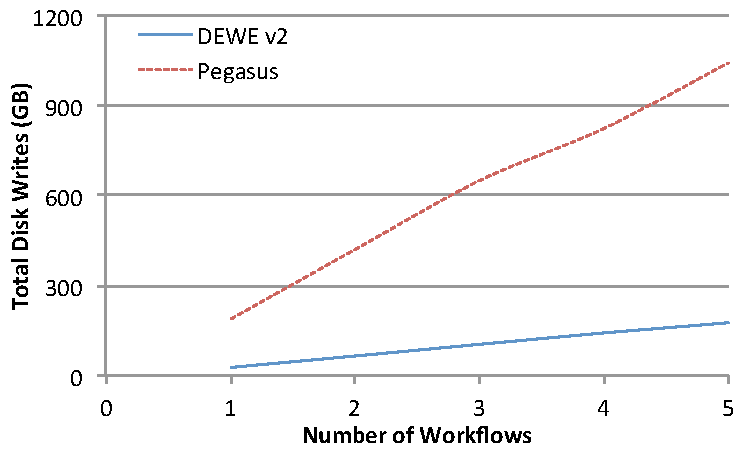
\includegraphics[width=6cm]{multi_run_disk_writes}} 
  \caption{Resource consumption of multiple 6.0 degree Montage Workflow running on a single-node cluster with Pegasus and DEWE v2. The instance type being used is c3.8xlarge.} 
  \vspace{-15pt}
  \label{fig:multi_run} 
\end{figure*}

In this paper, we use Pegasus as a representative of the scheduling-based workflow execution engines. 

Figure \ref{fig:compare_graphs} shows the resource consumption patterns of one 6.0 degree Montage workflow running on a single-node cluster with DEWE v2 and Pegasus. The experiments are carried out on AWS EC2 in its us-east-1 region. The instance type being used is c3.8xlarge. The storage being used is the instance-store SSD volumes with RAID 0 configuration. To eliminate the impact of network latency, the required input files are downloaded to the storage device before the experiments. Although the c3.8xlarge instance has 32 vCPU, the maximum number of concurrent threads observed is 25 for DEWE v2 and 20 for Pegasus. The maximum CPU utilization observed is 100\% for DEWE v2 and 80\% for Pegasus. This indicates that DEWE v2 is more efficient in utilizing CPU resources. The observed disk write operations for Pegasus is much higher than DEWE v2, indicating that Pegasus carries out more disk I/O activities than DEWE v2. For DEWE v2, the average makespan is 600 seconds. For Pegasus, the average make span is 1240 seconds, which is significantly longer. 

Figure \ref{fig:multi_run} shows the resource consumption of multiple 6.0 degree Montage workflows running on a single node cluster with Pegasus and DEWE v2. The instance being used  is c3.8xlarge on AWS EC2 in the us-east-1 region. The desired number of workflows are submitted to the workflow management system in one batch. The required input files are downloaded to the storage devices on the instance before the experiments. Total execution time (Figure \ref{fig:subfig:multi_run_makespan}) refers to the time needed to finish the execution of the workflows, regardless of the actual resource utilization rate on the worker nodes. When the number of workflows increases, the total execution time increases linearly. Total CPU time (Figure \ref{fig:subfig:multi_run_cpu_time}) refers to the actual CPU time spent on job execution activities, which is calculated by integrating the actual CPU utilization rate over the entire workflow execution period on all CPUs. Total disk writes (Figure \ref{fig:subfig:multi_run_disk_writes}) refers to the amount of data being written to the file system, which is calculated by integrating the actual disk write throughput over the entire workflow execution period. when the number of workflows increases, both total CPU time and total disk writes increase linearly. In general, Pegasus consumes a lot more computing resource (such as CPU time and disk writes) than DEWE v2, resulting in much longer execution time. For example, the execution time of five 6.0 degree Montage workflows being run with DEWE v2 is approximately the same as the execution time of one 6.0 degree Montage workflow being run with Pegasus. In other words, DEWE v2 can achieve 80\% speed-up when running multiple scientific workflows in parallel with the same cluster configuration. 



\subsection{Workflow Submission Intervals}
\label{sec:subsec:submission}


\begin{figure}[!t]
	\centering
	\hspace{-10pt}
	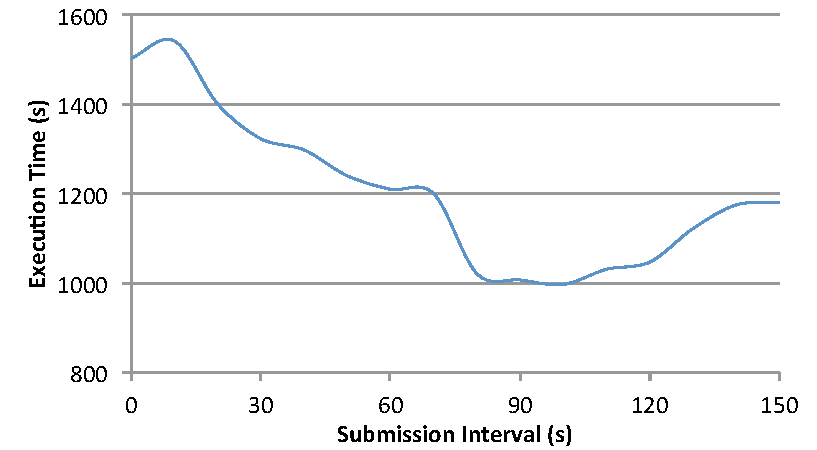
\includegraphics[width=8.5cm]{dewe_v2_submission_intervals}
    \vspace{5pt}
	\caption{Execution time of five 6.0 degree Montage Workflow running on a single-node cluster with DEWE v2. The instance type being used is c3.8xlarge.}
	\label{fig:dewe_v2_submission}
\end{figure}




A 6.0 degree Montage workflow demands different computing resources in different stages. When executing a large scale workflow ensemble with many workflows on the same cluster, it is possible to optimize resource utilization by controlling the workflow submission intervals so that different workflows in the workflow ensemble do not demand the same computing resource at the same time. In this test, we run a workflow ensemble with five 6.0 degree Montage workflows with DEWE v2 on a single-node cluster with both the master daemon and worker daemon on the same node. The test includes submitting all five workflows in one batch (batch submission), or submitting the five workflows one after another at fixed intervals (incremental submission). Batch submission can be considered as a special case of incremental submission where the submission interval is zero. As shown in Figure \ref{fig:dewe_v2_submission}, the time needed to execute all five workflows decreases when the submission interval increases, then increases again when the submission interval is greater than 100 seconds. In this particular test case, 34\% speed up can be achieved by setting the submission interval to 100 seconds.

Figure \ref{fig:dewe_v2_submission_pattern} shows the resource consumption patterns of the test workflow ensemble with five 6.0 degree Montage workflows running on a single node cluster with DEWE v2. Due to space limits we only show results with workflow submission intervals of 0, 50 and 100 seconds. As shown in Figure  \ref{fig:subfig:dewe_v2_submission_cpu}, when we increase the workflow submission interval, we change the CPU utilization pattern in the system. When submission interval is 0 second, the CPU utilization exhibits a clear three-stage pattern, with significant resource under-utilization in the second stage. This is very similar to the CPU utilization pattern in a single workflow. When submission interval is 100 seconds, such three-stage pattern is no longer obvious. This is because different types of jobs from different workflows can be executed in parallel, resulting in an increase in average CPU utilization across the whole execution time. The same result is also observed in disk I/O activities, which is reflected in both disk writes (Figure \ref{fig:subfig:dewe_v2_submission_disk_writes}) and disk reads (Figure \ref{fig:subfig:dewe_v2_submission_disk_reads}). Due to the increase in resource utilization, shorter execution time can be achieved with well-designed incremental submission techniques. 

\subsection{System Robustness}
\label{sec:subsec:rubustness}

We carry out two tests to examine the robustness of DEWE v2. In one test, we run one 6.0 degree Montage workflow with DEWE v2 on a single-node cluster with both the master daemon and worker daemon on the same node. During the execution of the workflow, we introduce interruptions to the system by killing the worker daemon and then starting it again 5 seconds later. In the other test, we run one 6.0 degree Montage workflow with DEWE v2 on a two-node cluster with NFS as the shared file system. One of the nodes has both the master daemon and the worker daemon, while the other node has only the worker daemon. However, at any time there is only one worker daemon running. During the execution of the workflow, we introduce interruptions to the system by killing the worker daemon on one node, then starting the worker daemon on the other node 5 seconds later. 

In both tests, interrupted jobs are automatically resubmitted for execution after timeouts. DEWE v2 is capable of completing the execution of the workflow, regardless of number of interruptions. When the interruptions are introduced during the execution of none-blocking jobs such as mProjectPP and mDiffFit, the increase in makespan roughly equals to the total duration of the interruptions. This is because DEWE v2 can resume execution of the workflow as soon as the worker daemon restarts, without the need to wait for the timeout of the interrupted jobs. When the interruptions are introduced during the execution of blocking jobs such as mConcatFit and mBgModel, the increase in makespan roughly equals to the sum of the timeout settings of the interrupted jobs. This is because DEWE v2 must wait for the timeout of the interrupted jobs to resume execution of the workflow.

DEWE v2's capability of resuming workflow execution after interruption of the worker daemon opens the door for dynamic resource provisioning. During the execution of large scale workflow ensembles, researchers can dynamically adjust the number of worker nodes in a cluster to meet both deadline and cost constrains. When there are a large number of none-blocking jobs in the queue, more worker nodes can be added to the cluster to speed up the execution. When there are a limited number of blocking jobs in the queue, some worker nodes can be removed from the cluster to reduce cost. Such dynamic resource provisioning strategy might not be effective for public clouds with a charge-by-hour model (such as AWS), but can be useful for public clouds with a charge-by-minute model (such as Google Compute Engine). In this paper, we carry out all our experiments on AWS, therefore we are not able to explore further on this topic.



\section{Resource Provisioning Strategy}
\label{v2_sec:provision}

\begin{figure*}[t!]
\centering
\vspace{-10pt}
 \subfloat[CPU Utilization]{ 
    \label{fig:subfig:dewe_v2_submission_cpu}  
    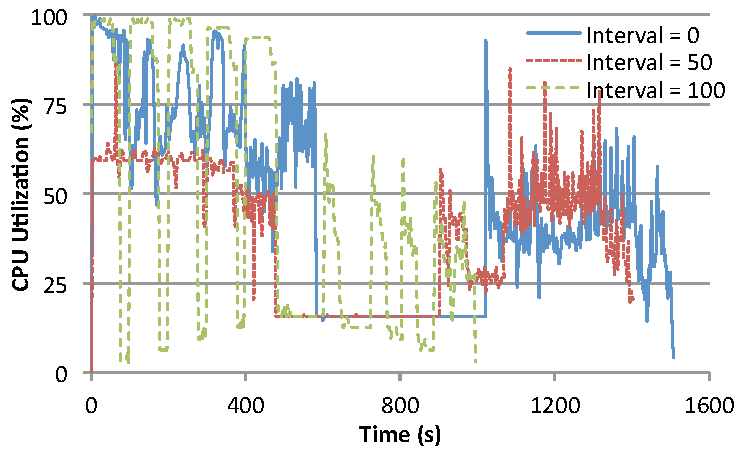
\includegraphics[width=6cm]{dewe_v2_submission_cpu}} 
  \hspace{5pt}
 \subfloat[Disk Write Operations]{ 
    \label{fig:subfig:dewe_v2_submission_disk_writes}  
    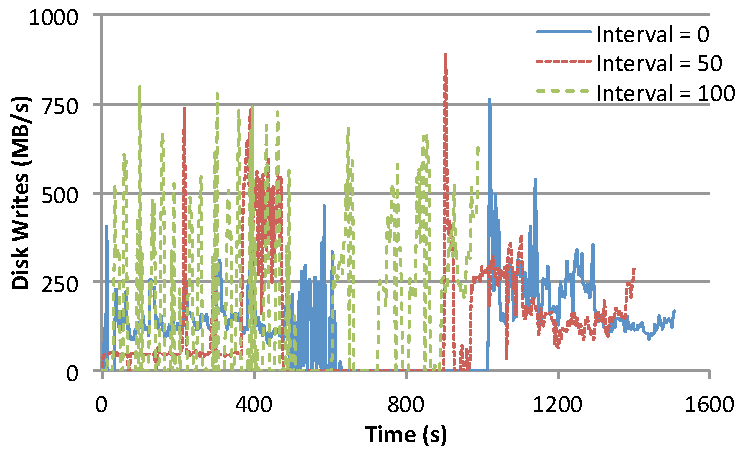
\includegraphics[width=6cm]{dewe_v2_submission_disk_writes}} 
  \hspace{5pt}
 \subfloat[Disk Read Operations]{ 
    \label{fig:subfig:dewe_v2_submission_disk_reads}  
    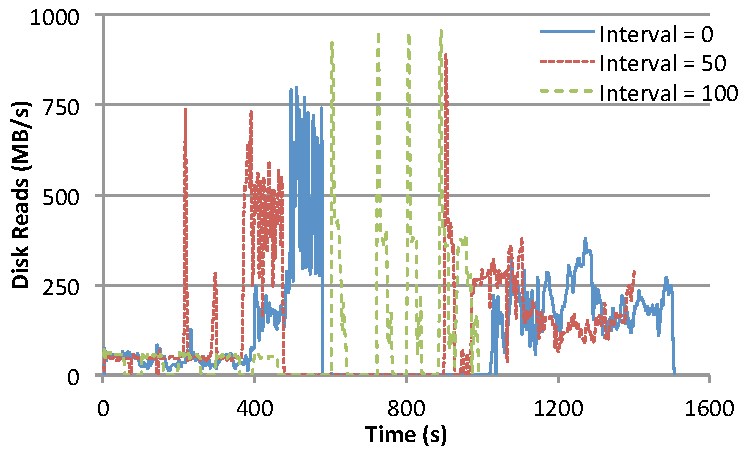
\includegraphics[width=6cm]{dewe_v2_submission_disk_reads}} 
  \caption{Resource consumption patterns of five 6.0 degree Montage workflows running on a single node cluster with DEWE v2. The workflow submission intervals are 0, 50 and 100 seconds.} 
  \label{fig:dewe_v2_submission_pattern} 
\end{figure*}

\begin{figure*}[t!]
\centering
\vspace{-10pt}
 \subfloat[CPU Utilization]{ 
    \label{fig:subfig:10_runs_cpu}  
    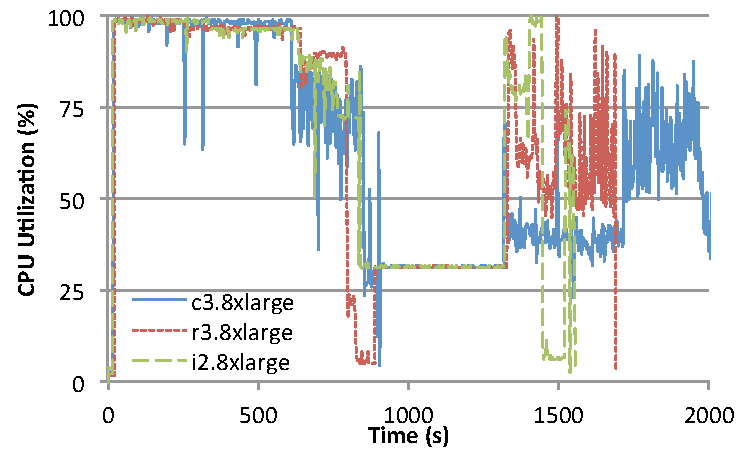
\includegraphics[width=6cm]{10_runs_cpu}} 
  \hspace{5pt}
 \subfloat[Disk Write Operations]{ 
    \label{fig:subfig:10_runs_disk_writes}  
    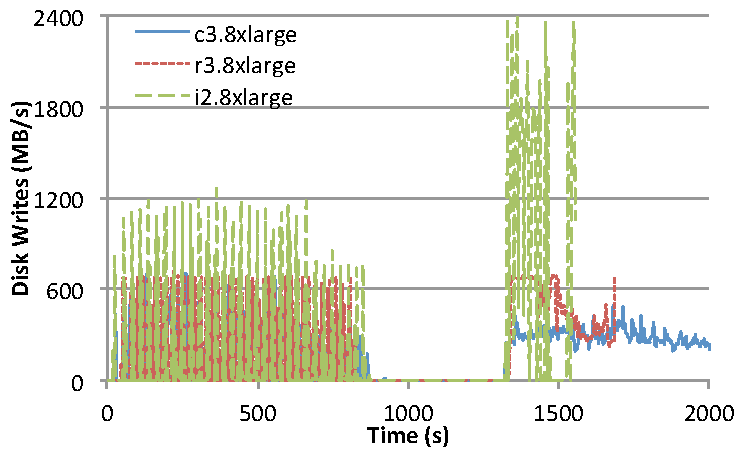
\includegraphics[width=6cm]{10_runs_disk_writes}} 
    \hspace{5pt}
 \subfloat[Disk Read Operations]{ 
    \label{fig:subfig:10_runs_disk_reads}  
    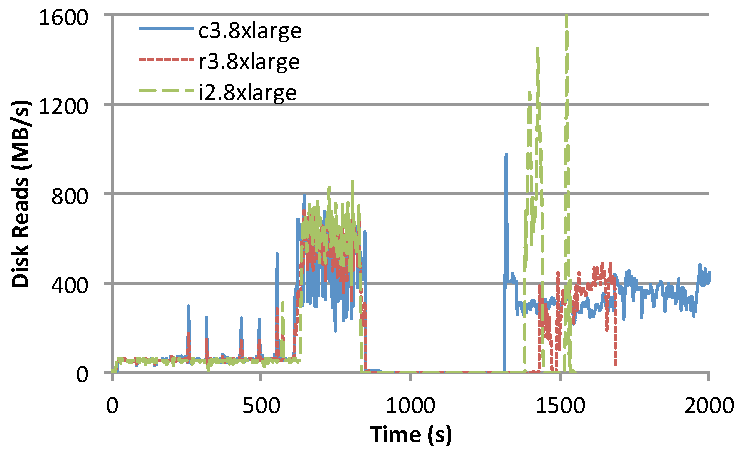
\includegraphics[width=6cm]{10_runs_disk_reads}} 
  \caption{Resource consumption patterns of ten 6.0 degree Montage workflows running on a single node cluster with DEWE v2. The instance type being used are c3.8xlarge, r3.8xlarge and i2.8xlarge.} 
  \label{fig:10_runs} 
\end{figure*}

In this section, we propose a two-step strategy to provision computing resources for large scale scientific workflow ensembles with both cost and deadline constraints. We begin with small scale experiments to profile the resource consumption patterns of the workflow ensemble when the underlying computing nodes are fully utilized. Based on the small scale testing results we derive the performance index of a worker node. Then we use the performance index to determine the number of worker nodes needed for the actual large scale experiments. To simplify our discussions, all the tests presented in this section are carried out with batch submission rather than incremental submission.

\subsection{Profiling}
\label{sec:subsec:pattern}

 
 \begin{figure*}[t!]
\centering
\vspace{-10pt}
 \subfloat[CPU Utilization]{ 
    \label{fig:subfig:2_node_cpu}  
    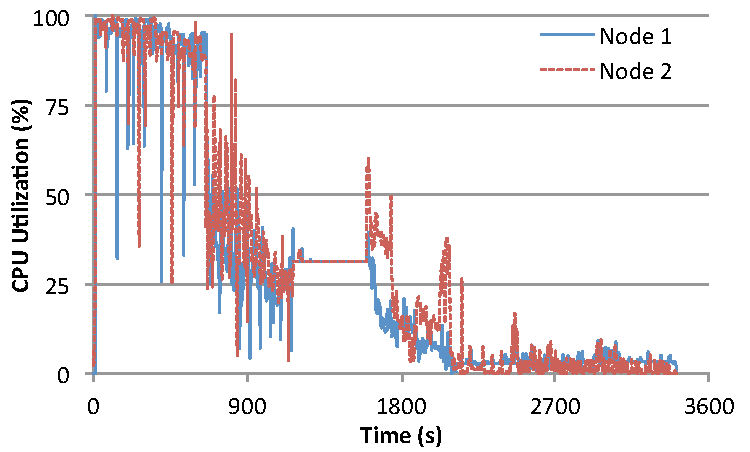
\includegraphics[width=6cm]{2_node_cpu}} 
  \hspace{5pt}
 \subfloat[Disk Write Operations]{ 
    \label{fig:subfig:2_node_disk_writes}  
    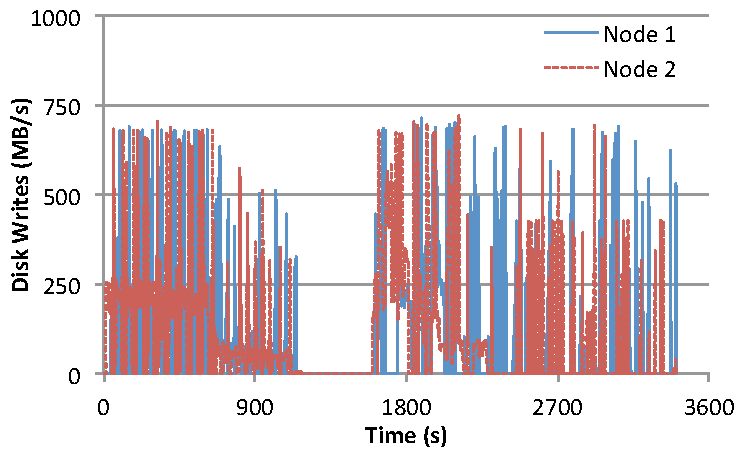
\includegraphics[width=6cm]{2_node_disk_writes}} 
  \hspace{5pt}
 \subfloat[Disk Read Operations]{ 
    \label{fig:subfig:2_node_disk_reads}  
    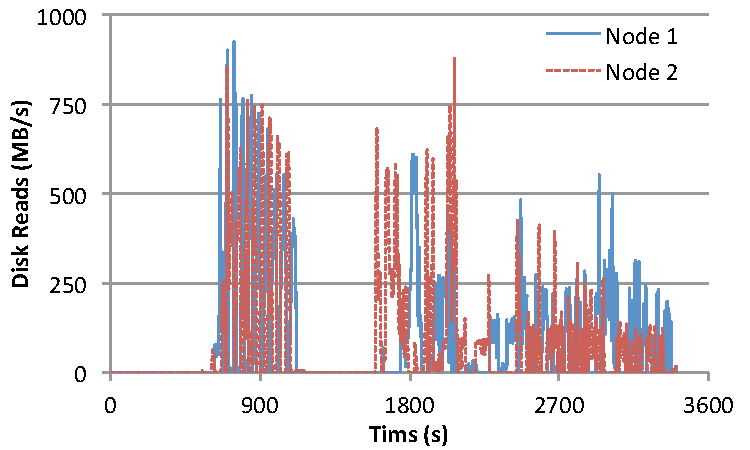
\includegraphics[width=6cm]{2_node_disk_reads}} 
\caption{Resource consumption patterns of 20 6.0 degree Montage workflows running on a 2-node cluster with DEWE v2. The instance type being used is r3.8xlarge. The shared file system is NFS.}   
  \label{fig:2_node_pattern} 
\end{figure*}

To come up with a resource provisioning strategy for executing large scale scientific workflow ensembles in public clouds, we use both single-node tests and multi-node tests to profile the resource consumption pattern of multiple workflows running in parallel. 


We use the c3.8xlarge, r3.8xlarge, and i2.8xlarge instances on AWS EC2 for our experiments. Table \ref{tbl:instance_type} lists the specifications of the selected instance types. On all of the selected instance types, the storage devices are SSD-backed instance store volumes (storage from disks that are physically attached to the host computer). To achieve the best disk I/O performance, we combine all the instance store volumes available on the instance in a RAID 0 configuration. All the workflow related disk I/O operations are configured to occur on the RAID 0 device. The file system being used on all worker nodes is ext4. Benchmark testings reveal that all three instance types have similar CPU and memory performance. However, there exists significant difference in the disk I/O performance of the RAID 0 device, which is shown in Table \ref{tbl:instance_disk_io}. 


In the single-node tests, we run up to ten 6.0 degree Montage workflows on a single-node cluster with DEWE v2. The largest workload contains 85,860 jobs, 14,440 input files with a total size of 40 GB, and 228,500 intermediate files with a total size of 350 GB. 

Figure \ref{fig:10_runs} shows the resource consumption pattern of ten 6.0 degree Montage workflows running on a single-node cluster with DEWE v2. During the first stage, the workflow is CPU intensive, as evidenced by the 100\% CPU utilization rate on all three instance types (Figure \ref{fig:subfig:10_runs_cpu}). If we look at the disk write operations alone (Figure \ref{fig:subfig:10_runs_disk_writes}), we would think that the workflow is I/O intensive during this stage. However, this stage takes approximately the same amount of time on all three instance types, regardless of the significant difference in their write throughput. This indicates that CPU is the real bottleneck during this stage. The operating system caches the disk writes and flushes them to the disk in batches, resulting in the intermittent disk writes at full capacity. During the second stage, the workflow is neither CPU intensive nor I/O intensive, as evidenced by the low CPU utilization rate and zero disk writes. The progress of the workflow is controlled by the single-thread mConcatFit and mBgModel jobs. During the third stage, the workflow is  I/O intensive. The i2.8xlarge instance, with the highest I/O capacity, finishes executing this stage first, following by the r3.8xlarge and the c3.8xlarge instances, according to their I/O capacities.




\begin{figure*}[t!]
\centering
\vspace{-10pt}
 \subfloat[Single-Node Cluster]{ 
    \label{fig:subfig:single_node_multi_runs}  
    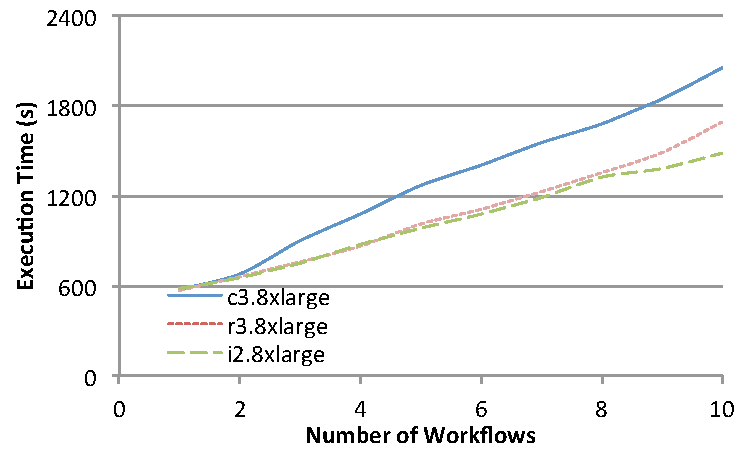
\includegraphics[width=6cm]{single_node_multi_runs}} 
  \hspace{5pt}
 \subfloat[Multi-Node Cluster]{ 
    \label{fig:subfig:multi_node_20_runs}  
    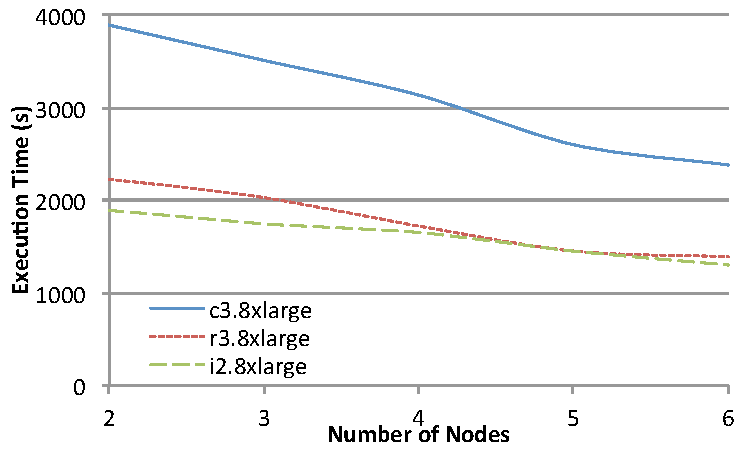
\includegraphics[width=6cm]{multi_node_20_runs}} 
  \hspace{5pt}
 \subfloat[Performance Degradation]{ 
    \label{fig:subfig:performance_degradation}  
    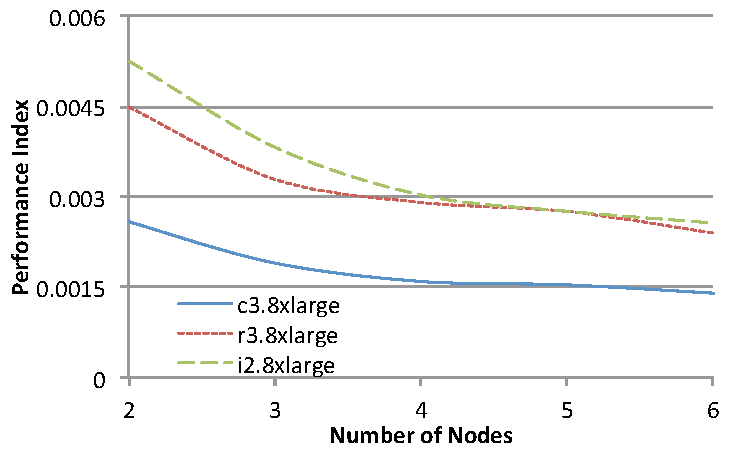
\includegraphics[width=6cm]{performance_index}} 
\caption{The impact of workload and cluster size on the performance of the cluster. On the single-node clusters, we run up to 10 6.0 degree Montage workflows. On the multi-node clusters, we run 20 6.0 degree Montage workflows in one batch.}   
  \label{fig:small_scale_summary} 
\end{figure*}

In the multi-node tests, we run twenty 6.0 degree Montage workflows on multi-node clusters with DEWE v2. The workload contains 172,720 jobs, 28,880 input files with a total size of 80 GB, and 457,000 intermediate files with a total size of 700 GB. In a multi-node cluster, one of the nodes runs both the master daemon and the worker daemon, while the other nodes run the worker daemon. All nodes share its storage with the other nodes using NFS. For example, in a two-node cluster, node A has a locally-mounted folder A and a NFS-mounted folder B, while node B has a NFS-mounted folder A and a locally mounted folder B. In order to balance the pressure on disk I/O, we evenly distribute the input files onto different nodes. For example, in a 2-node cluster, the input files for 10 workflows are located on node A while the input files for the other 10 workflows are located on node B.

Figure \ref{fig:2_node_pattern} shows the resource consumption pattern in a 2-node r3.8xlarge cluster. Similar to the resource utilization pattern in a single-node cluster, the first stage is controlled by the CPU resource and the second stage is controlled by the single-thread mConcatFit and mBgModel jobs. During the third stage, the CPU utilization on both nodes is extremely low, the progress of the workload is controlled by the large number of intermittent disk I/O operations. The peak of these I/O operations is 750 MB/s for both read and write operations, indicating the performance of NFS is the bottleneck of the cluster.  


\subsection{Determining Cluster Size}
\label{sec:subsec:Performance index}

Figure \ref{fig:small_scale_summary} shows the impact of workload and cluster size on the performance of the cluster. On the single-node cluster, the size of the cluster remains the same. As the number of workflows increases, the execution time increases linearly (Figure \ref{fig:subfig:single_node_multi_runs}). On the multi-node cluster, the size of the workload remains the same. As the number of worker nodes increases, the execution time decreases linearly (Figure \ref{fig:subfig:multi_node_20_runs}). 

The performance index of the worker nodes in a multi-node cluster can be defined as the execution speed of the workflow on a single node, that is

\begin{equation}
P =\frac{W}{N * T}
\label{eq:performance_index} 
\end{equation}
\\
where P is the performance index (workflow per second per node), W is the number of workflows running on the cluster, N is the number of worker nodes in the cluster, and T is the execution time needed for N workflows. A simple way to read this is how much of a workflow can be completed by one worker node in one second. As shown in Figure \ref{fig:subfig:performance_degradation}, as the number of worker nodes increases, the performance index decreases. The phenomenon is commonly observed in clusters, and is referred to as clustering performance degradation. In our test case, the observed clustering performance degradation gradually converges when the number of worker nodes is greater than 4. Based on Figure \ref{fig:subfig:performance_degradation}, we estimate that the performance indexes for large scale clusters are 0.0015, 0.0024, and 0.0026 for clusters with c3.8xlarge, r3.8xlarge, and i2.8xlarge instance types.

Based on Equation \ref{eq:performance_index}, we can estimate the number of worker nodes needed to execute a large scale scientific workflow ensemble with deadline constraints using the following formula:

\begin{equation}
N =\frac{W}{P * T}
\label{eq:node_estimation} 
\end{equation}
\\
where N is the desired number of worker nodes in the cluster, W is the number of workflows in the workflow ensemble, P is the performance index of the EC2 instance type, and T is the desired execution time. 



\subsection{Large Scale Experiments}
\label{v2_sec:subsec:large_scale}


\begin{table}[t!]
\caption{Cluster Configurations}
\label{tbl:cluster_config}
\centering
\begin{tabular}{|p{1.4cm}|p{0.9cm}|p{0.9cm}|p{0.9cm}|p{0.9cm}|p{0.9cm}|}
\hline
Cluster & Nodes & vCPU & Memory (TB) & Storage (TB)&Price (USD/hr)\\ \hline
c3.8xlarge & 40 & 1280 & 2.40 & 25.6 & 67.2\\ \hline
r3.8xlarge & 25 & 800  & 6.10 & 16.0 & 70.0\\ \hline
i2.8xlarge & 23 & 768  & 5.61 & 147.2 & 156.7\\ \hline
i2.8xlarge B & 10 & 320  & 2.44 & 64.0 & 68.2\\ \hline
\end{tabular}
\end{table}

\begin{figure*}[t!]
\centering
\vspace{-10pt}
 \subfloat[CPU Utilization]{ 
    \label{fig:subfig:large_scale_cpu}  
    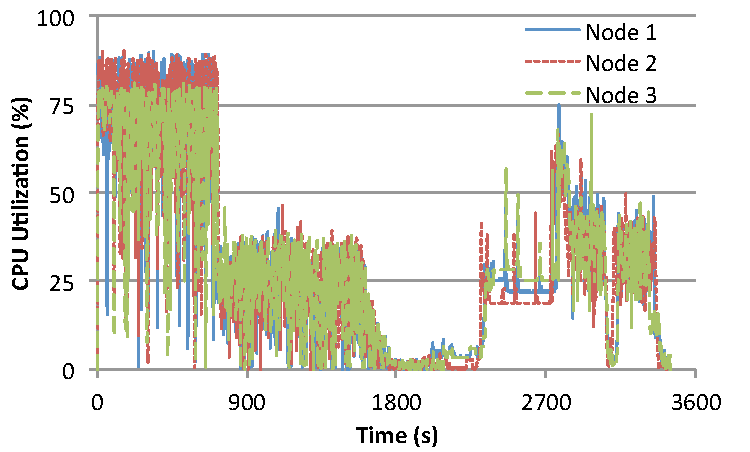
\includegraphics[width=6cm]{large_scale_cpu}} 
  \hspace{5pt}
 \subfloat[Disk Write Operations]{ 
    \label{fig:subfig:large_scale_disk_writes}  
    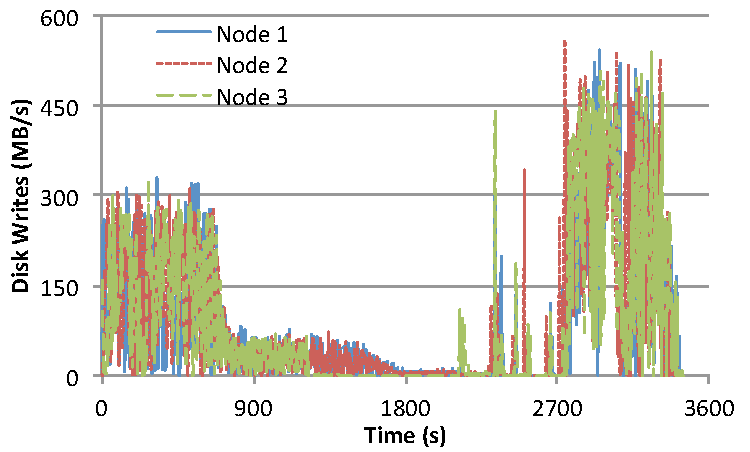
\includegraphics[width=6cm]{large_scale_disk_writes}} 
  \hspace{5pt}

 \subfloat[Disk Read Operations]{ 
    \label{fig:subfig:large_scale_disk_reads}  
    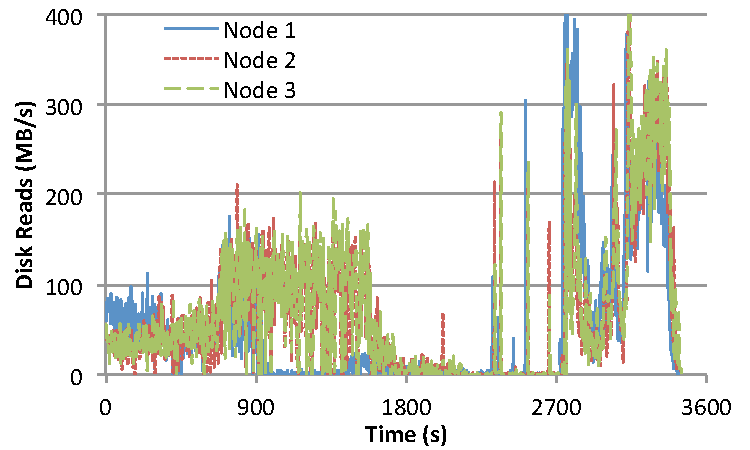
\includegraphics[width=6cm]{large_scale_disk_reads}} 
  \caption{Resource consumption patterns of 200 6.0 degree Montage workflows running on a 25-node cluster with DEWE v2. The instance type being used is r3.8xlarge.} 
  \label{fig:large_scale_pattern} 
\end{figure*}


\begin{figure*}[t!]
\centering
\vspace{-10pt}
 \subfloat[Execution Time]{ 
    \label{fig:subfig:large_scale_runs}  
    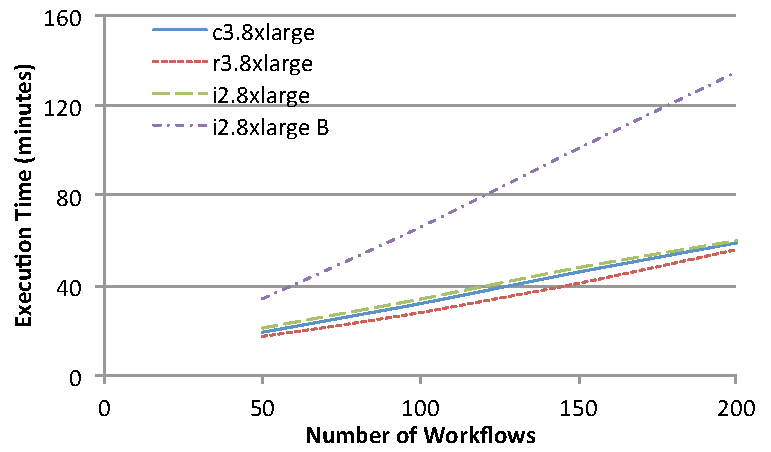
\includegraphics[width=6cm]{large_scale_runs}} 
  \hspace{5pt}
 \subfloat[Performance Index]{ 
    \label{fig:subfig:large_scale_performance}  
    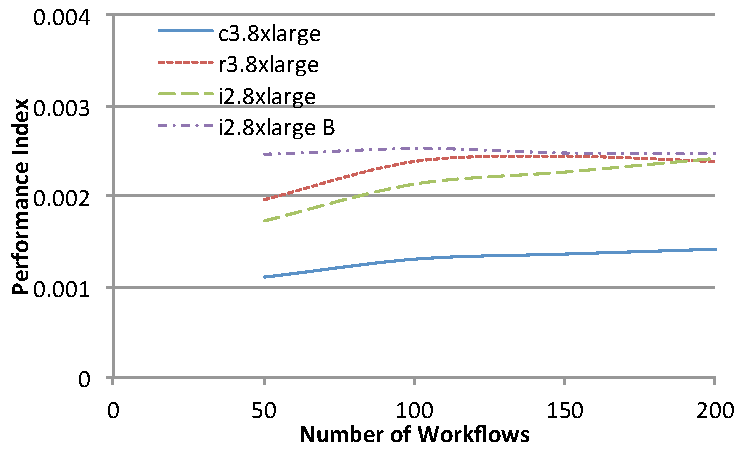
\includegraphics[width=6cm]{large_scale_performance_index}} 
  \hspace{5pt}
 \subfloat[Price per Workflow]{ 
    \label{fig:subfig:large_scale_price}  
    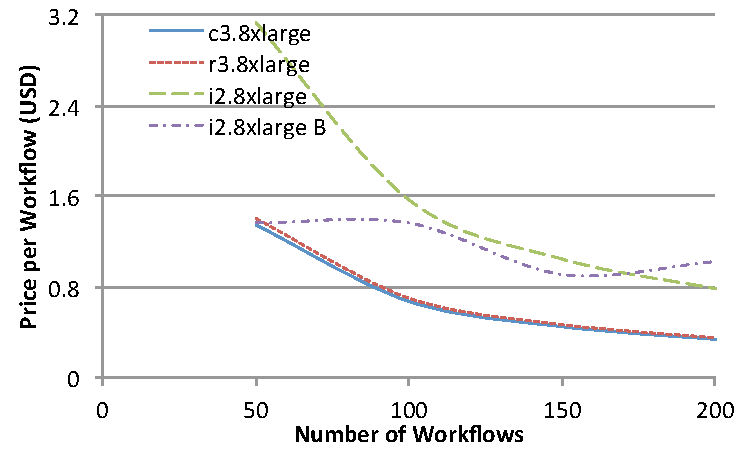
\includegraphics[width=6cm]{large_scale_price}} 
\caption{Summary of the large scale experiments.}   
  \label{fig:large_scale_runs} 
\end{figure*}

We use large scale experiments to evaluate the above-mentioned resource provisioning strategy. The largest workflow ensemble includes 200 6.0 degree Montage workflows, which contains 1,717,200 jobs, 288,800 input files, and 4,570,000 intermediate files. Approximately 7.0 TB data is written to the underlying storage during the execution. 

In order to meet both cost and deadline constraints, we design our clusters with the goal to complete the largest workload ensemble (W = 200) within an hour. This is because users pay for EC2 instances by the hour, and any partial hour usage will be charged as a full hour. The time constrain T is set to 3300 seconds (55 minutes) because we would like to have some flexibility in the execution time. Based on Equation \ref{eq:node_estimation}, the estimated number of worker nodes are 40, 25, and 23 for c3.8xlarge, r3.8xlarge and i2.8xlarge instance types. An additional cluster i2.8xlarge B with the i2.8xlarge instance type and 10 nodes is also tested as a comparison. We use 10 nodes for the i2.8xlarge B cluster because it has approximately the same hourly price as the c3.8xlarge and r3.8xlarge clusters. Table \ref{tbl:cluster_config} lists the four test clusters along with their total amount of vCPU, memory and storage, as well as the hourly price as calculated with the on-demand instance prices. 

In our previous experiments, we use NFS as the share file system between worker nodes. This requires each and every worker node to share its local storage via NFS, and mount the NFS shares from other nodes, resulting in an N-to-N mapping between worker nodes. As the size of the cluster grows, the configuration of the cluster becomes increasingly complex, resulting in unbalanced utilization. In the large scale experiments, we use MooseFS \cite{moosefs} as the shared file system between worker nodes. All the worker nodes are configured to be a MooseFS trunk server. Using cloud-init scripts, the worker nodes automatically join the storage pool and mount the MooseFS file system when the instances are being launched. Furthermore, the required input files are copied to the shared file system before the experiments. Therefore, the test results only include the execution time of the workflow ensemble. As a distributed file system, MooseFS has the option to store one file with multiple copies on different storage devices. In order to save storage space, each file has only one copy in our experiments. The worker nodes mount the shared file system as a POSIX-compliant file system. When executing a particular job, the worker daemon has no knowledge about the actual location of the input and output files. In order words, data locality can not be assumed in our experiments. However, it is safe to assume that statistically all worker nodes have equal access to the underlying shared file system. 


Figure \ref{fig:large_scale_pattern} shows the resource consumption pattern of 200 6.0 degree Montage workflows running on the r3.8xlarge cluster. The cluster includes 25 worker nodes, but we only present data from three worker nodes. As shown in the figure, all three worker nodes have the same the resource consumption patterns, which is similar to the resource consumption pattern on a single-node cluster (Figure \ref{fig:10_runs}). This is also true for other worker nodes not shown in the figure. This indicates that the workload is evenly distributed across the cluster. The cluster behaves in a way that is similar to a supercomputer. 


Figure \ref{fig:large_scale_runs} shows the execution time, performance index, and price per workflow for workflow ensembles with different number of 6.0 degree Montage workflows. For all clusters, the execution time increases linearly as the number of workflows in the workflow ensemble increases (Figure \ref{fig:subfig:large_scale_runs}). On clusters c3.8xlarge, r3.8xlarge and i2.8xlarge, the workflow ensemble with 200 6.0 degree Montage workflows is completed within 60 minutes, meeting the designed deadline constrain. On cluster i2.8xlarge B, the workflow ensemble with 200 6.0 degree Montage workflows takes 135 minutes to complete, significantly exceeding the designed deadline constrain.

Figure \ref{fig:subfig:large_scale_performance} shows the performance index for different clusters. The i2.8xlarge B cluster has the highest performance index. This is because the cluster has the smallest number of nodes, resulting in the highest resource utilization rate. For clusters c3.8xlarge, r3.8xlarge and i2.8xlarge, the performance index grows when the workload ensemble grows. When the number of workflows is small, the clusters are not fully utilized. In this case, the observed performance index is lower than the designed performance index. When the number of workflows is large, the clusters become fully utilized. In this case, the observed performance index is very close to the designed performance index. 


Figure \ref{fig:subfig:large_scale_price} shows the average price of executing a single workflow on different clusters under different workloads. For clusters c3.8xlarge, r3.8xlarge and i2.8xlarge, all the tests are completed in one hour. With the hourly pricing model, the cost is the same for different workloads. As a result, the price per workflow decreases as the workload increases. This suggests that the size of the cluster should be carefully designed based on the target workload to achieve the best price performance. For cluster i2.8xlarge B, the price per workflow fluctuates because the costs of running different workload are different. However, for the designed workload with 200 6.0 degree Montage workflows, all three clusters designed with the proposed resource provision model (c3.8xlarge, r3.8xlarge and i2.8xlarge) achieve lower price per workflow than cluster i2.8xlarge B, which is not designed with the proposed resource provision model. This indicates that the proposed resource provision strategy is effective in designing clusters to meet both cost and deadline constraints. 

\section{Disk IO Capacity}
\label{v2_sec:disk_io}



\begin{table*}[t!]
\caption{Disk I/O Performance of Modern HPC Systems \cite{borrill2009hpc}} 
\label{tbl:disk_io}
\centering
\begin{tabular}{|p{3.0cm}|p{1.2cm} | p{2.0cm}|p{1.2cm}| p{2.0cm} | p{2.0cm}|p{2.0cm}|}
\hline
Location & Cluster & Compute Cluster & File System & Storage System & Compute-Storage Interconnect & Measured Node Throughput (MB/s)\\ \hline
National Energy Research Scientific Computing Center & Franklin & Cray XT4 MPP with 38,128 nodes & Luster & 96 storage targets & Cray SeaStar-2 & 1200 \\ \hline
Oak Ridge National Laboratory  & Jaguar & Cray XT5 with 18,680 nodes & Luster & 672 storage targets & Cray SeaStar-1 & 1200 \\ \hline
Lawrence Livermore National Laboratory  & Thunder & Itanium2 with 1024 nodes & Luster & 32 storage targets & Quadrics Elan4 & 400 \\ \hline
Lawrence Berkeley National Laboratory & Bassi & Power5 with 122 nodes & GPFS & 24 IBM DS4300 storage systems & IBM HPS Federation & 6100 \\ \hline
Lawrence Berkeley National Laboratory & Jacquard & Opteron with 320 nodes & GPFS & 672 storage targets & InfiniBand & 1200 \\ \hline
Argonne National Labs & Intrepid & BG/P with 8192 nodes & GPFS & 16 IBM x3655 file servers & 10 GigE & 300 \\ \hline
Argonne National Labs & Surveyor & BG/P with 1024 nodes & PVFS2 & 1 IBM x3655 file servers & 10 GigE & 200 \\ \hline
\end{tabular}
\end{table*}


In the large scale experiments with 200 6.0 degree Montage workflows, DEWE v2 is able to write 7.0 TB of data to the MooseFS distributed file system within 60 minutes. On cluster r3.8xlarge, all worker nodes are able to perform intensive disk I/O operations at the throughput of over 500 MB/s concurrently to the shared file system. The estimated aggregate throughput for the r3.8xlarge cluster is 12.5 GB/s. 

Table \ref{tbl:disk_io} shows the disk I/O performance of the parallel file system in modern HPC systems \cite{borrill2009hpc}. The measured node throughput of our r3.8xlarge cluster exceeds the measured node throughput of clusters Intrepid and Surveyor at Argonne National Labs, as well as cluster Thunder at Lawrence Livermore National Laboratory. In other words, the disk I/O performance of the the distributed file system on r3.8xlarge cluster on AWS EC2 is comparable to the disk I/O performance of the parallel file system in modern HPC systems. Therefore, public cloud is a viable option for executing large scale disk I/O intensive scientific workflow ensembles.


\section{Summary}
\label{v2_sec:summary}

In this chapter, we address two main challenges in executing large-scale workflow ensembles in public clouds: (1) execution coordination, and (2) resource provisioning. We present our solutions to these challenges with the development of DEWE v2, a pulling-based workflow management system, and its effective resource provisioning strategy. 

By adopting the pulling approach in our solution system, we have demonstrated that much of scheduling overhead when executing a large-scale workflow ensemble particularly in public clouds can be removed as a majority of tasks in scientific workflows often exhibit homogeneity in their resource consumption pattern and acquiring a large number of homogeneous public cloud resources is easily possible. We compare the performance of DEWE v2 with Pegasus showing DEWE v2 is capable of achieving 80\% speed-up. We have also demonstrated that provisioning cloud resources using our profiling-based strategy based on performance index is very effective in terms of both cost and deadline compliance.

In experiments with a single 6.0 degree Montage workflow, DEWE v2 is capable of achieving 50\% speed-up as compared to Pegasus. In experiments with Montage workflow ensembles, DEWE v2 is capable of achieving 80\% speed-up as compared to Pegasus. This demonstrates that the pulling approach has better performance over the scheduling approach in executing large scale scientific workflow ensembles in public clouds. In the case of workflow ensembles, further speed-up can be achieved using workflow job submission techniques as opposed to batch submission in DEWE v2.

For large scale workflow ensembles, the optimal amount of computing resources can be calculated using the concept of performance index, which is derived from profiling applications in small scale testings. The largest workflow ensemble tested includes 200 6.0 degree Montage workflows, which contains 1,717,200 jobs, 288,800 input files, and 4,570,000 intermediate files. Approximately 7.0 TB data is written to the underlying storage during the execution. Small scale testings with 20 6.0 degree Montage workflows (10\% of the large scale experiment) are used to derive the performance indexes of different EC2 instance types. The derived performance indexes is then used to calculate the number of worker nodes needed for the large scale experiments. This technique is proven to be effective in meeting both cost and deadline constraints. 





\chapter{Conclusion}
\label{chapter:conclusion}

In this study, we address two main challenges in executing large-scale workflow ensembles in public clouds: (1) execution coordination, and (2) resource provisioning. We present our solutions to these challenges with the development of DEWE v2, a pulling-based workflow management system, and its effective resource provisioning strategy. 
By adopting the pulling approach in our solution system, we have demonstrated that much of scheduling overhead when executing a large-scale workflow ensemble particularly in public clouds can be removed as a majority of tasks in scientific workflows often exhibit homogeneity in their resource consumption pattern and acquiring a large number of homogeneous public cloud resources is easily possible. We compare the performance of DEWE v2 with Pegasus showing DEWE v2 is capable of achieving 80\% speed-up. We have also demonstrated that provisioning cloud resources using our profiling-based strategy based on performance index is very effective in terms of both cost and deadline compliance.











%%%%%%%%%%%%
% End

% Bibliography
\bibliographystyle{style/mybibstyle}
{
\setstretch{1.25}
\cleardoublepage
\phantomsection
\bibliography{references}
}

%%%% Appendices
%%%\appendix
%%%\addtocontents{toc}{\protect\setcounter{tocdepth}{1}}
%%%\input{wikifeats/wikifeats.tex}
%%%\input{candcner/candcner.tex}
%%%\input{comparedata/comparedata.tex}

\end{document}